\documentclass[master]{finthesis}

\usepackage[pdftex]{graphicx}
\usepackage{amsmath}

\usepackage{caption}
\usepackage{subcaption}
\captionsetup[figure]{font=footnotesize, justification=centering}
\captionsetup[table]{font=footnotesize, justification=centering}
\usepackage{tikz}
\usepackage{circuitikz}
%\usetikzlibrary{through, patterns}
%\usepackage{tikzscale}

%\usepackage[T1]{fontenc}

\usepackage[dvipsnames]{xcolor} % for more colors
\usepackage{amssymb} % for arrow symbol
\usepackage{tikz, pgfplots} % for diagram
\usepackage{schemabloc}  % for tikz trapezium
\usepackage{booktabs} % for bold lines in table
\usepackage{fancyhdr} % for header and footer
\usepackage{float}
\usepackage{placeins}

% For group PGF plots
\pgfplotsset{compat=newest}
\usetikzlibrary{pgfplots.groupplots}
\usepgfmodule{oo}

\makeatletter
\newcommand*{\engl}[2][\@empty]{%
    \edef\theacronym{#1}%
    (енгл. \foreignlanguage{english}{\emph{#2}%
    \ifx\theacronym\@empty \else , #1\fi})%
}
\makeatother

% Color variables
\def \CtrlColor        {darkgray}
\def \BBctrlColor      {RoyalBlue}
\def \PIDctrlColor     {OliveGreen}
\def \DCOColor         {BrickRed}
\def \CtrlDecColor     {brown}
\def \CtrlPreprocColor {RoyalPurple}
\def \ClkDivColor      {Goldenrod}
\def \RstnColor        {BurntOrange}

% Abbreviation variables
\def \PLL  {PLL} % phase-locked loop
\def \FLL  {FLL} % frequency-locked loop
\def \DLL  {DLL} % delay-locked loop
\def \DCO  {DCO} % digitally controlled oscillator 
\def \PID  {PID} % proportional-integral-derivative
\def \P    {P}   % proportional
\def \I    {I}   % integral
\def \D    {D}   % derivative
\def \FCW  {FCW} % frequency control word
\def \PVT  {PVT} % process-voltage-temperature
\def \HLLS {HLLS} % high-low level shifter
\def \LHLS {LHLS} % low-high level shifter


\addbibresource{master_rad.bib}

\title{Пројектовање синтетизабилне сведигиталне фреквенцијски затворене петље са широким опсегом подешавања до учестаности од 640\texorpdfstring{\,}{ }MHz}
\author{Ђорђе С. Гачић}
\studid{408/2022}
\advisor{проф. др Владимир М. Миловановић}
\advisorfull{Др Владимир М. Миловановић,\\ванредни професор}

\studprog{Електротехника и рачунарство}
% \module{Модул}
\course{Напредно машинско учење}
\date{\today}
% \date{ГГГГ-ММ-ДД}

\committee{др Шћепан Шћекић}
\committee{доц. др Жарко Попара}

\studentshould{% У оквиру овог рада кандидат треба да...
}

%\titlepagebib{greenwade93}
%\titlepagebib{pythonsite}
\titlepagebib{Staszewski:FREQUENCY_SYNTHESIZER_CMOS_2005}
\titlepagebib{Razavi:PLL_CMOS_2020}

\thesisapplicationfile{slike/prijava}

\abstracten{Frequency-locked loop (FLL) represents a viable way of generating a range of frequencies from a single reference frequency by using a negative feedback electronic control system that compares the frequency of a controlled oscillator to the reference one. A digital synthesizable FLL is designed in 130\,nm CMOS technology for a target frequency of up to 640\,MHz. It employs a wide-tuning range digitally controlled oscillator (DCO) assembled from tri-state inverters in the form of a matrix. The FLL can optionally use a bang-bang or a soft-programmable standard proportional-integral-derivative (PID) controller to regulate the feedback loop. Its design practically minimizes metastability occurrence. The proposed digital FLL occupies 100\,\textmu m $\times$ 330\,\textmu m and consumes 3.5\,mW in typical operating conditions. The reference clock is 16\,MHz, and the output oscillation frequency is set to 640\,MHz, while the achieved frequency resolution is 2.8\,MHz.}
\keywordsen{Frequency-locked loop, digitally controlled oscillator, clock generator, synthesizable, CMOS technology, PID controller, metastability}

\abstractsr{Фреквенцијски затворена петља \engl[FLL]{Frequency-Locked Loop} представља одржив начин генерисања опсега фреквенција из једне референтне фреквенције коришћењем електронског система управљања са негативном повратном спрегом, који пореди фреквенцију контролисаног осцилатора са поменутом референтном фреквенцијом. Дигитално синтетизабилан \FLL\ је дизајниран у 130\,nm технологији за циљану фреквенцију до 640\,MHz. Он погони дигитално контролисани осцилатор \engl[DCO]{Digitally Controlled Oscillator} са широким подешавањем опсега који се састоји од тростатаичких инвертора у облику матрице. \FLL\ може произвољно користити тзв. \engl{Bang-Bang} контролер или дјелимично програмирани стандардни пропорционално, интегрални, диференцијални \engl[PID]{Proportional-Integral-Derivative} контролер за управљање негативном петљом. Такав дизајн у пракси минимизује појаву метастабилности. Предложени дигитални \FLL\ заузима 100\,\textmu m $\times$ 330\,\textmu m простора и троши 3.5\,mW у уобичајеним условима рада. Референтни такт је 16\,MHz, а излазна фреквенција осциловања је подешена на 640\,MHz, док постигнута резолуција фреквенције износи 2.8\,MHz.}
\keywordssr{Фреквенцијски затворена петља, дигитално контролисани осцилатор, генератор такта, синтетизабилност, CMOS технологија, \PID\ контролер, метастабилност}

% Semantic markup. Look it up!
%\newcommand{\cmd}[2][]{\texttt{\textbackslash #2#1\{\ldots\}}} % Well, this one is useful beyond just semantics...
%\newcommand{\env}[1]{\texttt{#1}}
%\newcommand{\pkg}[1]{\texttt{#1}}
%\newcommand{\prog}[1]{\texttt{#1}}

\begin{document}

\maketitle

\tableofcontents

\makeabstract

\section{Увод}
У данашње вријеме, фазно затворена петља \engl[PLL]{Phase-Locked Loop} и петља са затвореним кашњењем \engl[DLL]{Delay-Locked Loop} представљају свеприсутне блокове у дизајну чипова. Безброј примјена самих чипова захтјевају или генератор такта или синтетизатор фреквенције, што подразумјева уградњу неког од поменутих блокова унутар система који се пројектује. Главна улога таквог блока у дизајну је да генерише стабилан и прецизан излазни сигнал чија је фаза подесива у односу на фазу улазног сигнала, самим тим одржавајући везу између улазне и излазне фреквенције. Међутим, чак и веома сложени системи често захтјевају генератор такта, који само множи улазну фреквенцију без да посебно води рачуна о фази такта или апсолутном подрхтавању \engl{Jitter}. У таквим примјенама, потребна и довољна је само фреквенцијски затворена петља \engl[FLL]{Frequency-Locked Loop} да би се испунили тражени захтјеви.

По дефиницији, \FLL\ је управљачки систем са негативном повратном спрегом који закључава фреквенцију излазног сигнала на предвиђену циљану фреквенцију. У принципу, непрастано управља фреквенцијом осцилатора на аутоматски начин све док излазна фреквенција на достигне циљану вриједност, након чега се та вриједност фреквенције одржава на излазу. Постоје многи начини имплементације \FLL-а~\cite{Ali:9097205}. Штавише, \FLL\ као интегрисано коло може спадати у двије групе: дигитални и аналогни \FLL. Иако је очигледан недостатак првих максимална фреквенција и њена резолуција, они посједују многе друге предности наспрам њихових аналогних супарника. Они заузимају мање простора, истичу се већом отпорношћу на промјене процесних углова, напона и температуре \engl[PVT]{Process-Voltage-Temperature}, лако су употребљиви у различитим технологијама, и стога омогућавају поновну употребу, већу прилагодљивост, једноставнију методологију тока пројектовања, као и брже циклусе пројектовања. Узимајући у обзир све претходно поменуто, испоставља се да је у општем случају боље ићи ка развоју дигиталног \FLL-a кад год спецификација архитектуре система то дозвољава. Дакле, фокус овог рада је пројектовати и унаприједити једноставне али моћне синтетизабилне дигиталне блокове чипа.

Овај рад конкретно предлаже синтетизабилан дигитални \FLL\ сличан предложеном у литератури~\cite{Musa:6644316}, са побољшаном брзином закључавања \FLL-а~\cite{Deng:6891375} и смањеним ризиком од метастабилности. Осцилатор је састављен од тростатичких инвертора и заснован на прстенастом \DCO-у из литературе~\cite{Tierno:4443210} измјењен додавањем независног напона напајања \DCO-а са претварачима напонских нивоа \engl{Level Shifters} и употребом петостепене~\cite{Rylyakov:4523284} умјесто тростепене толологије прстена осцилатора.

Остатак рада укључује додатна поглавља. Поглавље \ref{FLL structure} описује предложени дигитални \FLL\ на системском нивоу и нивоу блокова и кола уз детаљна теоријска разматрања. Поглавље \ref{Implementation and results} пружа увид у имплементацију и добијене резултате симулација, такође уз теоријска разматрања појава које су од значаја за рад читавог система. Коначно, поглавље \ref{Conclusion} закључује рад и наговјештава могућности даљег рада на побољшању и проширењу система.


\section{Структура фреквенцијски затворене петље} \label{FLL structure}


У овом раду описана је релативно једноставна али ефикасна дигитална фреквенцијски затворена петља (\FLL). чију се системску архитектуру на нивоу блокова приказује \figurename~\ref{FLL block diagram}. Описани \FLL\ се практично састоји из два блока: дигитално контролисаног осцилатора (\DCO) и блока управљачке логике, који генерише улазне сигнале за \DCO\ на основу тренутне фреквенције \DCO-a. У сврху поједностављења, са слике су изостављени неки конфигурациони улази \FLL-a, као што су умножак фреквенције \engl[FCW]{Frequency Control Word}, коефицијенти \PID\ контролера и улаз за одабир режима рада. 

% FLL block diagram
\begin{figure*}[ht]
	\centering
	\begin{tikzpicture}[thick, scale=0.53, every node/.style={scale=0.45}]
		% Grid
		%\draw[step=1cm, gray, very thin] (0,0) grid (40,10);
		% Setup
		%\tikzset{every node/.style={align=center}};
		%\tikzstyle{every node}=[draw]
		% Beginning
		\draw                         (0  ,0) -- (0  ,5);
		\draw [-]                     (0  ,5) -- (1  ,5);
		\draw [-,  \CtrlColor]        (1  ,5) -- (1.5,5);
		\draw [->, \CtrlPreprocColor] (1.5,5) -- (1.94  ,5);
		% Preprocessing stage (grey counter + gra2bin conversion + synchronization)
		\node (GREYCNT)  at (2.8,5) [draw, \CtrlPreprocColor, minimum size=2cm, minimum height=2.4cm, align=center]{ГРЕЈЕВ  \\ БРОЈАЧ \\[5pt] \framebox{1,3,2,6}};
		\node (CONVSYNC) at (5.8,5) [draw, \CtrlPreprocColor, minimum size=2cm, minimum height=2.4cm, align=center]{СИНХР. \\ БИНАРНИ \\ ПРЕТВАРАЧ \\[5pt] \framebox{$\rightleftarrows$}};
		\draw [->, \CtrlPreprocColor] (GREYCNT) -- (CONVSYNC);
		\draw [dashed, \CtrlPreprocColor, fill=\CtrlPreprocColor, fill opacity=0.1, text opacity=1] (1.5,3.5) rectangle (7.5,6.5) node[midway, above=0.85]{УПРАВЉАЧКА ПРЕДОБРАДА};
		% Splitter/demultiplexer
		\node (DEMUX) at (8.5,5) [draw, \CtrlColor, trapezium, trapezium stretches=true, minimum width=7cm, minimum height=1cm, rotate=90]{ДЕМУЛТИПЛЕКСЕР};
		\draw [-,  \CtrlPreprocColor] (CONVSYNC) -- (7.5,5);
		\draw [->, \CtrlColor]           (7.5,5) -- (DEMUX);
		% Bang-bang FLL control branch
		\draw [-,    \CtrlColor]  (9  ,6.5) -- ( 9.5,6.5);
		\draw [->, \BBctrlColor] ( 9.5,6.5) -- (10  ,6.5);
		\node (CMP) at (11.4,6.5) [draw, \BBctrlColor, minimum size=2cm, minimum height=2.4cm, align=center]{КОМПАРАТОР \\[5pt] \framebox{$\geq$}};
		\node (CNT) at (14.2,6.5) [draw, \BBctrlColor, minimum size=2cm, minimum height=2.4cm, align=center]{БРОЈАЧ \\[5pt] \framebox{1,2,3}};
		\draw [->, \BBctrlColor]      (CMP) --      (CNT);
		\draw [-,  \BBctrlColor]      (CNT) -- (15.5,6.5);
		\draw [->,   \CtrlColor] (15.5,6.5) -- (16  ,6.5);
		\draw [dashed, \BBctrlColor, fill=\BBctrlColor, fill opacity=0.1, text opacity=1] (9.5,5) rectangle (15.5,8) node[midway, above=0.85]{ДВОСТЕПЕНИ РЕГУЛАТОР};
		% PID FLL control branch
		\draw [->, \CtrlColor] ( 9,3.5) -- (11,3.5);
		\node (PID) at (12.5,3.5) [draw, \PIDctrlColor, fill=\PIDctrlColor, fill opacity=0.1, text opacity=1, minimum width=3.5cm, minimum height=2.4cm, align=center]{\PID\ \\ РЕГУЛАТОР \\[5pt]};
		\draw [\PIDctrlColor] plot[smooth] coordinates {(11.75,2.7) (12.0,3.2) (12.5,3.1) (13.25,3.1)};
		\draw [\PIDctrlColor, fill=\PIDctrlColor, fill opacity=0.1] (11,2.5) rectangle (14,4.5) node[midway, below=0.6, opacity=1] {};
		\draw [->, \CtrlColor] (14,3.5) -- (16,3.5);
		% Control logic box
		\draw [dashed, \CtrlColor, fill=\CtrlColor, fill opacity=0.1, text opacity=1] (1,1) rectangle (21,9) node[midway, above=2.15]{УПРАВЉАЧКА ЛОГИКА};
		% Multiplexer
		\node (MUX) at (16.5,5) [draw, \CtrlColor, trapezium, trapezium stretches=true, minimum width=7cm, minimum height=1cm, rotate=-90]{МУЛТИПЛЕКСЕР};
		% Control Decoder
		\node (CTRLDEC) at (19,5) [draw, \CtrlDecColor, fill=\CtrlDecColor, fill opacity=0.1, text opacity=1, minimum size=2cm, minimum height=2.4cm, align=center]{УПРАВЉАЧКИ \\ ДЕКОДЕР};
		\draw [->, \CtrlColor] (MUX)  -- (CTRLDEC);
		% DCO
		\node (DCO) at (23,5) [draw, \DCOColor, fill=\DCOColor, fill opacity=0.1, text opacity=1, minimum size=2.4cm, minimum height=2.4cm, align=center]{DCO \\[5pt]};
		\draw [\DCOColor](22.8,4.7) sin (22.9,4.8) cos (23.0,4.7) sin (23.1,4.6) cos (23.2,4.7);
		\draw [\DCOColor](23.0,4.7) circle (0.3);
		\draw [-, \CtrlColor] (CTRLDEC) -- (21,5);
		\draw [->]                     (21,5) --  (DCO);
		% End
		\draw  (DCO) -- (25,5);
		\draw (25,5) -- (25,0);
		\draw (25,0) --  (0,0);
		
        \draw (-1,-1) rectangle (26,10) node[midway, above=2.95]{\textbf{ДИГИТАЛНА ФРЕКВЕНЦИЈСКИ ЗАТВОРЕНА ПЕТЉА}};	
        \draw [thick, ->] (-2.5,9) -- (-1,9) node[midway, above=0.1] {\textbf{RSTN}};
        \draw [thick, ->] (-2.5,8) -- (-1,8) node[midway, above=0.1] {\textbf{FREF}};        	
        \draw [thick, ->] (-2.5,7) -- (-1,7) node[midway, above=0.1] {\textbf{FMUL}};
        \draw [thick, ->] (-2.5,6) -- (-1,6) node[midway, above=0.1] {\textbf{CTRL}};
        \draw (-2.0,6.825) --  (-1.5,7.175);
        \draw (-2.0,5.825) --  (-1.5,6.175);
        %\draw [-]  (25,5) -- (26,5);
        \draw [thick, ->] (26,8) -- (27.5,8) node[midway, above=0.1] {\textbf{FOUT}};
        \draw [thick, ->] (26,7) -- (27.5,7) node[midway, above=0.1] {\textbf{LOCK}};
        
		
	\end{tikzpicture}
	\caption{Блок дијаграм дигиталне фреквенцијски затворене петље састављене од: блока управљачке логике (лијево) и дигитално контролисаног осцилатора (десно).}
	\label{FLL block diagram}
\end{figure*}


\subsection{Управљачка логика дигиталне фреквенцијски затворене петље}
Управљачка логика \FLL-a састоји се од двије независне процесне гране, које представљају два међусобно искључива режима управљања \FLL-a. Оба режима на улазу примају бинарну вриједност повезану са бројем периода такта \DCO-а унутар периода референтног такта. Такође, оба управљачка режима генеришу бинарну вриједност на излазу, која представља управљачку бинарну ријеч осцилатора директно пропорционалну излазној фреквенцији. Главне разлике између два поменута режима су брзина затварања (закључавања) \FLL-a и једноставност подешавања. Циљ управљачке логике \FLL-a је изједначити вриједност улазног множача фреквенције са бројем периода такта \DCO-a унутар периода референтног такта што је брже и прецизније могуће одрадити, чиме се долази до постизања жељене фреквенције на излазу \DCO-a. Комплетна управљачка логика \FLL-a је подијељена на неколико фаза, које су описане у наредним поглављима.

\subsubsection{Управљачка предобрада}
Фаза управљачке предобраде \engl{Control Preprocessing} укључује неколико блокова чија је функција претворити информацију о фреквенцији излазног такта \DCO-a у бинарну вриједност која ће бити прослијеђена као улаз наредној фази управљачке логике \FLL-a. Као прво, да би се одредила брзина осциловања \DCO-a, потребан је бројач. У имплементацији описаној у овом раду коришћен је Грејев бројач умјесто природног бинарног бројача из разлога што значајно умањује метастабилност бројача изазвану узорковањем \engl{Sampling}, јер у Грејевом коду свака узастопна вриједност се разликује за по један бит. Недостатак овог приступа је то што Грејев бројач има мању максималну радну фреквенцију од бинарног бројача. Да би се у још већем обиму смањио ризик од метастабилности, сваки бит са излаза Грејевог бројача се пропушта кроз синхронизатор са два флип-флопа да би безбједно прешао у подручје референтног такта. Затим, синхронизована вриједност Грејевог бројача се претвара у бинарни формат и узоркује се за даљу обраду.
% TODO
% Нешто више о Грејевом бројачу

\subsubsection{Bang-bang контролер}
Први управљачки блок \FLL-a је веома сличан bang-bang (или on-off) контролеру, односно контролеру са повратном спрегом који, као прекидач, може имати два стања. Он пореди улазни умножак фреквенције са узоркованом вриједношћу бројача и одлучује да ли инкрементирати, декрементирати или онемогућити предстојећи блок тј. двосмјерни бројач \engl{Up-Down Counter}. То осигурава постепено управљање и закључавање све до постизања жељене фреквенције.

% TODO
% Нешто више о bang-bang контролеру

\subsubsection{\PID~контролер}
У другом управљачком режиму, управљачка бинарна ријеч за \DCO\ се генерише подесивим \PID\ контролером. \PID\ контролер је управљачки механизам заснован на повратној спрези, који ради тако што непрекидно исправља и скалира сигнал грешке, који је разлика између измјерене вриједности у обради (узоркована вриједност бројача) и жељене референтне задате вриједности (вриједност улазног умношка фреквенције). Исправљање и скалирање се распоређује у три компоненте: пропорционална (\P), интегрална (\I) и диференцијална (\D), имплементиране као подесиви улази са фиксном тачком који се напајају из банке регистара. \par
Сврха \P\ компоненте је да управља брзином одзива управљачког система, непосредно множећи сигнал грешке константним чиниоцем. \I\ компонента се користи за смањење грешке стабилног стања \engl{Steady State} скалирањем грешке константним чиниоцем и сумирањем резултата током времена. \D\ компонента пропорционална брзини промјене грешке, и њен циљ је ограничити излаз да би се смањила могућа прекорачења или осцилације узроковане \P\ и \I\ компонентама, без смањења брзине контролера. Како је у овом систему референтна задата вриједност константна и нема брзих промјена на улазу које могу изазвати такав исход, \P\ и \I\ компоненте су довољне за гладак и стабилан одзив система.  

% TODO
% Нешто више о PID контролеру

\subsubsection{Управљачки декодер} \label{control decoder}
Улога управљачког декодера је претворити управљачке податке из једне бинарне вриједности у скуп управљачких улаза \DCO-а. Постоје три таква улаза: \textit{Row On}, унарни вектор, који може да укључује само читаве редове тростатичких инвертора \DCO-a; \textit{Row Select}, један од $n$ вектор \engl{One-Hot Vector}, који укључује један додатни ред тростатичких инвертора \DCO-a; и \textit{Column Select}, унарни вектор, који може да укључује колоне тростатичких инвертора \DCO-a. Да би се један инвертор укључио, или \textit{Row On}, или и \textit{Row Select} и \textit{Column Select} за одговарајући бит морају бити подешени на 1. Ширина сваког вектора је једнака ширини улаза. Сама структура \DCO-a је детаљније описана у поглављу \ref{DCO structure}.

% TODO
% Нешто више о унарном и један од n кодирању

\subsection{Структура дигитално контролисаног осцилатора} \label{DCO structure}
У срцу сваке фазно затворене петље се налази осцилатор који игра кључну улогу у учинку који може бити постигнут~\cite{Razavi:PLL_CMOS_2020}. Дигитално контролисани осцилатор описан у овом раду је прстенасти осцилатор, погодан за систем генерисања такта. Прстенасти осцилатор је каскадна комбинација фаза кашњења повезаних у ланац затворене петље~\cite{Madhusudhana:283751064}. Прстенасте архитектуре су компактније од LC осцилатора и имају доста предности захваљујући својој правилној и периодичној просторној структури. Уопштена структура \DCO-а коришћеног унутар описаног \FLL-а заснована је на матрици тростатичких CMOS инвертора~\cite{Terosiet:340277809}. Ова матрица је састављена од $N$-фазних прстена тростатичких инвертора повезаних паралелно. $N$ представља број \DCO\ фаза (степени) и мора бити непаран број већи или једнак 3.
%(за осцилатор са једним излазним сигналом у односу на заједничко уземљење)
У физичком смислу, матрица може бити преобликована у квадрат, што омогућава једноставнију управљачку логику. Један или више прстенова су увијек укључени и дефинишу основну фреквенцију \DCO-а. Остали тростатички инвертори се укључују и искључују у зависности од управљачке логике. \par
Формула за фреквенцију осциловања конкретне имплементације \DCO-а из овог рада гласи:
\begin{equation} \label{f_osc}
    f_\text{osc} = \dfrac{1}{2Nt_\text{d}} \approx \dfrac{I_\text{d}}{2NC_\text{load}V_\text{DDL}},
\end{equation} \\
гдје је $N$ број тростатичких инвертора унутар прстена, $t_\text{d}$ представља кашњење једне ћелије \DCO-a, у чијем саставу је тростатички инвертор (у наставку ће бити детаљније објашњена структура саме ћелије \DCO-а), $I_\text{d}$ је струја која протиче кроз инвертор, $C_\text{load}$ је капацитивно оптерећење истог инвертора, и $V_\text{DDL}$ је напон напајања \DCO-а. Производ $Nt_\text{d}$ је помножен са $2$ да би се добила читава периода такта, а не полупериода.

\subsubsection{Предложена архитектура DCO-a}
Када је рijеч о топологији, са повећањем броја \DCO\ фаза (степени), фреквенцијски корак ($K_\text{DCO}$) опада, чиме се повећава прецизност \DCO-а. Максимална фреквенција осцилатора се се такође смањује, и да би се то надомјестило, напон напајања се може повећати, што с друге стране доводи до веће потрошње снаге. Ако претпоставимо да напон напајања и капацитивно оптерећење по једној фази остану непромјењени, повећање броја фаза не утиче на потрошњу снаге. Међутим, ако укупан број тростатичких инвертора остане непромјењен и подијели се на већи број фаза, то ће довести до смањења капацитивног оптерећења по фазама појединачно, што даље доводи до смањења потрошње снаге. Математичком анализом се то може објаснити на следећи начин: $N$-фазни прстенасти осцилатор који ради на фреквенцији $f_\text{osc}$ има динамичку потрошњу снаге која се може представити једначином
\begin{equation} \label{dynamic power}
    	P = N f_\text{osc} C_\text{tot} V^{2}_\text{DDL}, 
\end{equation}
гдје $C_\text{tot}$ представља укупно капацитивно оптерећење на једној фази. Пошто је фреквенција осциловања једнака
\begin{equation}
	f_\text{osc} = \frac{1}{2Nt_\text{d}},
\end{equation}
једначину за динамичку снагу можемо написати на следећи начин:
\begin{equation}
    	P = \frac{C_\text{tot}V^{2}_\text{DDL}}{2t_\text{d}},
\end{equation}
одакле се види да је добијена динамичка снага независна од $N$~\cite{Razavi:PLL_CMOS_2020}. \par

У овом раду описана је топологија \DCO-a са пет фаза, због тога што је таквом топологијом остварен задовољавајући компромис између учинка и потрошње снаге. \figurename~\ref{DCO5} приказује структуру \DCO-а коришћеног у описаној \FLL\ имплементацији. 
\pgfooclass{InvRow}{
    \method InvRow(){}
    \method apply(#1,#2,#3){
        \draw 
        (#1,#2) node[ieeestd not port, anchor=in, scale=0.4, fill=ColorPhase0, fill opacity=\InvFillOpacity]({#3}0){}
        ({#3}0.out) node[ieeestd not port, anchor=in, scale=0.4, fill=ColorPhase1, fill opacity=\InvFillOpacity]({#3}1){}
        ({#3}1.out) node[ieeestd not port, anchor=in, scale=0.4, fill=ColorPhase2, fill opacity=\InvFillOpacity]({#3}2){}
        ({#3}2.out) node[ieeestd not port, anchor=in, scale=0.4, fill=ColorPhase3, fill opacity=\InvFillOpacity]({#3}3){}
        ({#3}3.out) node[ieeestd not port, anchor=in, scale=0.4, fill=ColorPhase4, fill opacity=\InvFillOpacity]({#3}4){};
    }
}
\begin{figure*}[!ht]
\centering
\begin{tikzpicture}[scale=0.95]
    \ctikzset{tripoles/mos style/arrows}
    \ctikzset{tripoles/pmos style/emptycircle}
    \ctikzset{logic ports=ieee}

    \definecolor{ColorPhase0}{RGB}{255,0,0}
    \definecolor{ColorPhase1}{RGB}{192,0,64}
    \definecolor{ColorPhase2}{RGB}{128,0,128}
    \definecolor{ColorPhase3}{RGB}{64,0,192}
    \definecolor{ColorPhase4}{RGB}{0,0,255}

    \definecolor{HLLSColor}{RGB}{64,0,77}
    \definecolor{LHLSColor}{RGB}{106,0,128}

    \definecolor{AlwaysOnBoxColor}{RGB}{0,255,0}
    
    % Color opacity variables
    \def \InvFillOpacity      {1}
    \def \DCOFillOpacity      {0.05}
    \def \CtrlDecFillOpacity  {0.1}
    \def \AlwaysOnBoxOpacity  {0.1}
    \def \HLLSFillOpacity     {0.1}
    \def \HLLSTextOpacity     {1}
    \def \LHLSFillOpacity     {0.05}
    \def \LHLSTextOpacity     {1}
    %
    \pgfoonew \invRow=new InvRow()
    %
    % LEFT INVERTER MATRIX
    \invRow.apply(0,0,i0)
    \invRow.apply(0,0.8,i1)
    \invRow.apply(0,1.6,i2)
    %
    \foreach \x in {0,1,2,3,4}
        \draw ({i0}\x.out) -- ({i1}\x.out) -- ({i2}\x.out) --++ (0,0.5) node[anchor=west, rotate=90, scale=0.5](lcont\x){...};
    \draw ({i0}0.in) -- ({i1}0.in) -- ({i2}0.in) --++ (0,0.5) node[anchor=west, rotate=90, scale=0.5](lcont5){...};
    %
    \invRow.apply(0,3,i3)
    \invRow.apply(0,3.8,i4)
    \invRow.apply(0,4.6,i5)
    %
    \foreach \x in {0,1,2,3,4}
        \draw (lcont\x.east) -- ({i3}\x.out) -- ({i4}\x.out) -- ({i5}\x.out);
    \draw (lcont5.east) -- ({i3}0.in) -- ({i4}0.in) -- ({i5}0.in);
    %
    % RIGHT INVERTER MATRIX
    \invRow.apply(5.8,0,ii0)
    \invRow.apply(5.8,0.8,ii1)
    \invRow.apply(5.8,1.6,ii2)
    %
    \foreach \x in {0,1,2,3,4}
        \draw ({ii0}\x.out) -- ({ii1}\x.out) -- ({ii2}\x.out) --++ (0,0.5) node[anchor=west, rotate=90, scale=0.5](rcont\x){...};
    \draw ({ii0}0.in) -- ({ii1}0.in) -- ({ii2}0.in) --++ (0,0.5) node[anchor=west, rotate=90, scale=0.5](rcont5){...};
    %
    \invRow.apply(5.8,3,ii3)
    \invRow.apply(5.8,3.8,ii4)
    \invRow.apply(5.8,4.6,ii5)
    %
    \foreach \x in {0,1,2,3,4}
        \draw (rcont\x.east) -- ({ii3}\x.out) -- ({ii4}\x.out) -- ({ii5}\x.out);
    \draw (rcont5.east) -- ({ii3}0.in) -- ({ii4}0.in) -- ({ii5}0.in);
    %
    % RECTANGLE FOR ALWAYS ON INVERTERS
    \draw 
    ({i0}0.in) ++ (-0.2,-0.4) node[](ron1){}
    ({i0}0.in) ++ (-0.2,0.4) node[](ron2){}
    ({ii0}4.out) ++ (0.2,0.4) node[](ron3){}
    ({ii0}4.out) ++ (0.2,-0.4) node[](ron4){};
    \filldraw[draw, AlwaysOnBoxColor, fill=AlwaysOnBoxColor, fill opacity=\AlwaysOnBoxOpacity] (ron1.center) -- (ron2.center) -- (ron3.center) -- (ron4.center) -- (ron1.center);
    %
    % UPPER PHASE CONNECTIONS
    \draw ({i5}4.out) ++ (0,1.1) |-++ (0,0.2) node[circ, scale=0.4](circ1){} --++ (0.5,0) node[anchor=west, scale=0.5](contp0){...}
    (contp0.east) -| ({ii5}4.out);
    \draw [dashed] ({i5}4.out) --++ (0,1.1);
    \draw [dashed] ({ii5}0.in) --++ (0,1.1);
    \draw ({ii5}0.in) ++ (0,1.1) --++ (0,0.2) node[circ, scale=0.4](circ2){}
    ({i5}0.in) |- (circ1);
    \foreach \x/\y in {0/1, 1/2, 2/3, 3/4} {
        \draw 
        (contp\x.west) ++ (0,-0.2) node[anchor=west, scale=0.5](contp\y){...}
        ({i5}\x.out) |- (contp\y.west)
        (contp\y.east) -| ({ii5}\x.out);
    }
    \draw
    ({i4}4.out) ++ (0.5,0) node[anchor=west, scale=0.5](contc0){...}
    ({i1}4.out) ++ (0.5,0) node[anchor=west, scale=0.5](contc1){...};
    %
    % BOTTOM ARROWS FOR ALL INVERTERS
    \foreach \r in {0,1,2,3,4,5}{
        \foreach \c in {0,1,2,3,4}{
            \draw ({i\r}\c.down) node[inputarrow, rotate=90, scale = 0.8]{} --++ (0,-0.3);
            \draw ({ii\r}\c.down) node[inputarrow, rotate=90, scale = 0.8]{} --++ (0,-0.3);
        };
    };
    %
    % DCO RECTANGLE
    \draw
    ({i0}0.in) ++ (-0.5,-1.2) node[](r1){}
    ({i5}0.in) ++ (-0.5,1.6) node[](r2){}
    ({ii5}4.out) ++ (0.5,1.6) node[](r3){}
    ({ii0}4.out) ++ (0.5,-1.2) node[](r4){}
    (r1) node[anchor=south west](){DCO};
    \filldraw[draw, \DCOColor, fill=\DCOColor, fill opacity=\DCOFillOpacity] (r1.center) -- (r2.center) -- (r3.center) -- (r4.center) -- (r1.center);
    %
    % COLUMN CONTROL RECTANGLE
    \draw
    (r2) ++ (0.5,1.8) node[](rc1){} 
    (r3) ++ (-0.5,1.8) node[](rc4){}
    (rc1) ++ (0,0.5) node[](rc2){}
    (rc4) ++ (0,0.5) node[](rc3){}
    ($(rc1)!0.5!(rc4)$) node[anchor=south, scale=0.8, text=\CtrlDecColor]{Управљање колонама};
    \filldraw[draw, \CtrlDecColor, fill=\CtrlDecColor, fill opacity=\CtrlDecFillOpacity] (rc1.center) -- (rc2.center) -- (rc3.center) -- (rc4.center) -- (rc1.center);
    %
    % HLLS FROM COLUMN CONTROL RECTANGLE
    \foreach \i/\x in {0/0.4, 1/1.15, 2/1.9, 3/2.65, 4/3.4, 5/6.2, 6/6.95, 7/7.7, 8/8.45, 9/9.2} {
        \draw
        (rc1) ++ (\x,0) --++ (0,-0.4) node[inputarrow, rotate=-90](){} node[rectangle, minimum size=3, thick, rotate=-90, anchor=west, scale=0.7, color=HLLSColor, fill=HLLSColor, fill opacity=\HLLSFillOpacity, text opacity=\HLLSTextOpacity, draw](hl\i){HLLS}
        (hl\i.east) --++ (0,-0.4) node[inputarrow, rotate=-90](){};
    }
    \draw
    (hl4.north) ++ (0.67,0) node[anchor=west, scale=0.5](){...}
    %
    % ROW CONTROL RECTANGLE
    (r1) ++ (-1.8,1.6) node[](rr1){} 
    (r2) ++ (-1.8,-1.2) node[](rr4){}
    (rr1) ++ (-0.5,0) node[](rr2){}
    (rr4) ++ (-0.5,0) node[](rr3){}
    ($(rr1)!0.5!(rr4)$) node[anchor=north, scale=0.8, rotate=-90, text=\CtrlDecColor]{Управљање редовима};
    \filldraw[draw, \CtrlDecColor, fill=\CtrlDecColor, fill opacity=\CtrlDecFillOpacity] (rr1.center) -- (rr2.center) -- (rr3.center) -- (rr4.center) -- (rr1.center);
    %
    % HLLS FROM ROW CONTROL RECTANGLE
    \foreach \i/\y in {0/0.4, 1/1.2, 2/2.5, 3/3.3, 4/4.1} {
        \draw
        (rr1) ++ (0,\y) --++ (0.4,0) node[inputarrow](){} node[rectangle, minimum size=3, thick, anchor=west, scale=0.7, color=HLLSColor, fill=HLLSColor, fill opacity=\HLLSFillOpacity, text opacity=\HLLSTextOpacity, draw](hlr\i){HLLS}
        (hlr\i.east) --++ (0.4,0) node[inputarrow](){};
    }
    \draw 
    (hlr1.north) ++ (0,0.3) node[anchor=west, rotate=90, scale=0.5](){...}
    %
    % LHLS AND PHASE PORTS
    ($(r3)!0.5!(r4)$) node[](rph2){}
    (rph2) ++ (0,0.7) node[](rph1){}
    (rph1) ++ (0,0.7) node[](rph0){}
    (rph2) ++ (0,-0.7) node[](rph3){}
    (rph3) ++ (0,-0.7) node[](rph4){};
    %
    \foreach \i in {0,1,2,3,4} {
        \draw
        (rph\i.center) --++ (0.4,0) node[inputarrow](){} node[rectangle, minimum size=3, thick, anchor=west, scale=0.7, color=LHLSColor, fill=LHLSColor, fill opacity=\LHLSFillOpacity, text opacity=\LHLSTextOpacity, draw](lh\i){LHLS} 
        (lh\i.east) --++ (0.4,0) node[signal, anchor=west, fill=ColorPhase\i, draw](ph\i){} node[inputarrow](){}
        (ph\i.east) node[anchor=west, scale=0.8]{Фаза \i};
    }
\end{tikzpicture}
\caption{Петостепени прстенасти дигитално контролисани осцилатор (\DCO) састављен од тростатичких инвертора, са додатим претварачима напонских нивоа (\HLLS\ и \LHLS) и уоквиреним редом стално укључених тростатичких инвертора.}
\label{DCO5}
\end{figure*}
 \par
Свака фаза \DCO-а састоји се од 54 тростатичка инвертора, што ако помножимо са бројем фаза даје укупно 270 инвертора. Тростатички инвертори су распоређени у 18 редова и 15 колона. Управљачка логика \FLL-a управља са 17 редова и свих 15 колона, што значи да постоји 255 фреквенцијских корака. Преостали ред са 3$\times$5 тростатичких инвертора је увијек укључен и на њега не утиче управљачка логика \FLL-а. Што се више тростатичких инвертора у свакој фази укључи под утицајем управљачке логике \FLL-а, тренутна снага покретања \engl{Driving Strength} једне фазе се повећава, док њено капацитивно оптерећење у суштини остаје константно, што резултује повећањем излазне фреквенције осциловања~\cite{Tierno:4443210}.

\subsubsection{Блок дијаграм DCO ћелије}
Да би се ефикасно подесила излазна фреквенција \DCO-а, уведен је скуп управљачких улаза \DCO-а, а то су сигнали \textit{Row On}, \textit{Row Select} и \textit{Column Select}, поменути такође у секцији \ref{control decoder}. Према томе, сваки тростатички инвертор појединачно садржи сопствену управљачку јединицу у облику И-ИЛИ стандардне ћелије, и заједно граде већи блок назван ћелија \DCO-а. \figurename~\ref{DCO_cell} приказује шему ћелије \DCO-а на нивоу логичких кола и на нивоу CMOS транзистора.
\begin{figure}[!ht]
    \centering
    %\vspace{0.7cm}
    \subfloat[]{
    \begin{tikzpicture}[scale=1]
        \ctikzset{tripoles/mos style/arrows}
        \ctikzset{tripoles/pmos style/emptycircle}
        \ctikzset{logic ports=ieee}
        \draw (0,0)
        node[ieeestd not port, anchor=out, scale=1](tsinv){}
        (tsinv.in) --++ (-0.5,0) node[signal, anchor=east, scale=1, draw](pinphi){} 
        (pinphi.west) node[anchor=east, scale=1]{In}
        %(tsinv.in) --++ (0,-1.3) --++ (-8.5,0) node[anchor=east, scale=1](inlong){In}
        %(inlong) --++ (-0.5,0) node[signal, anchor=east, scale=1, draw](pinphi){} 
        (tsinv.out) --++ (0.4,0) node[signal, anchor=west, scale=1, draw](pinpho){} 
        (pinpho.east) node[anchor=west, scale=1]{Out}
	(tsinv.up) --++ (0,0.4) node[anchor=west, scale=1]{ctrl} |-++ (-3.5,0.2) node[ieeestd not port, anchor=out, scale=1](not) {} 
	(tsinv.down) --++ (0,-0.4) node[anchor=west, scale=1]{$\overline{\mbox{ctrl}}$}
	(not.in) --++ (-1,0) node[ieeestd nor port, anchor=out, scale=1](nor){}
        (nor.in 2) -|++ (0, -0.6) node[ieeestd and port, anchor=out, scale=1](and){}
        (nor.in 1) -- (and.in 1|-nor.in 1) node[signal, anchor=east, scale=1, draw](pinro){} 
        (pinro.west) node[anchor=east, scale=1]{Row On}       
        (and.in 1) node[signal, anchor=east, scale=1, draw](pinrs){} 
        (pinrs.west) node[anchor=east, scale=1]{Row Sel.}
        (and.in 2) node[signal, anchor=east, scale=1, draw](pincs){} 
        (pincs.west) node[anchor=east, scale=1]{Col. Sel.};
	\draw[-] (not.in) node[circ]{} --++ (0,-1.8) -| (tsinv.down);
	\draw[dashed] (and.in 2) ++ (0.2,0) node[](csin){} --++ (0,2.5) -| (not.out) --++ (0,-2.9) -| (csin);
	\draw[dashed] (not.in) ++ (-0.3,0) node[](notin){} --++ (0,1) -| (tsinv.out) --++ (0,-1.7) -| (notin);
	\draw (csin) ++ (2.5,2.5) node[anchor=south west](andorlabel){\small И-ИЛИ}; 
	\draw (csin) ++ (7,2.1) node[anchor=south west](tsinvlabel){\small Тростатички инвертор}; 
	%\draw[dashed] (not.out) --++ (0,0.9);
	\draw[thick] (tsinv.down) node[draw, circle, anchor=north, fill=white, minimum size=0.17cm, inner sep=0] (invup) {};
        %\draw[decoration={brace, mirror},decorate] (not.out) ++ (0,0.9) --++ (-3.25,0) node[above=2pt] {\small И-ИЛИ} --++ (-3.23,0);
    \end{tikzpicture}
    %\vspace{0.2cm}
    \label{DCO_cell_logic_gate_level}
    }
    \vfil
    %\hfil
    \vspace{0.5cm}
    \subfloat[]{
    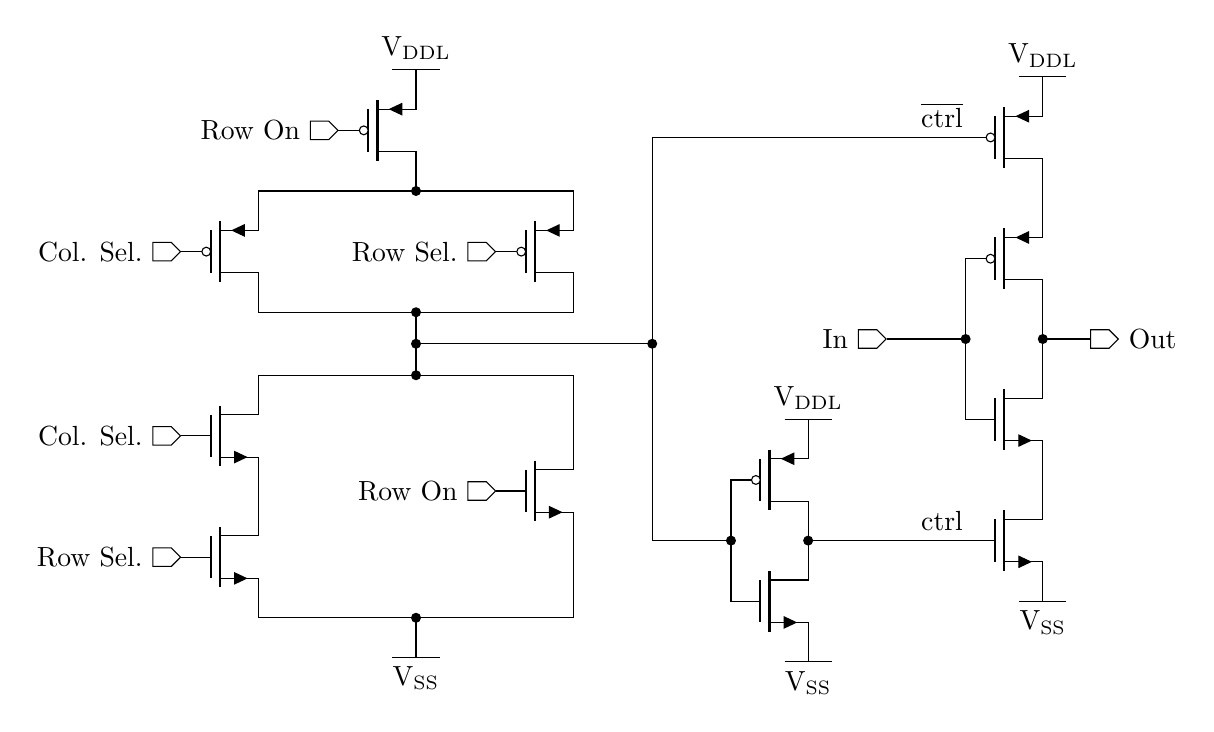
\begin{tikzpicture}[scale=1]
        \ctikzset{tripoles/mos style/arrows}
        \ctikzset{tripoles/pmos style/emptycircle}
        \ctikzset{logic ports=ieee}
        \draw (0,0)
        node[pmos, scale=1](pmos1){}
        (pmos1.D) to [short] ++(0,-0.5) node[nmos, scale=1, anchor=D](nmos1){}
        (pmos1.G) to (nmos1.G)
        ($(pmos1.G)!0.5!(nmos1.G)$) node[circ, scale=1]{} --++ (-1,0) node[signal, anchor=east, scale=1, draw](pinphi){} 
        (pinphi.west) node[anchor=east, scale=1]{In}
        ($(pmos1.D)!0.5!(nmos1.D)$) node[circ, scale=1]{} --++ (0.6,0) node[signal, anchor=west, scale=1, draw](pinpho){} 
        (pinpho.east) node[anchor=west, scale=1]{Out}
        (pmos1.S) node[pmos, scale=1, anchor=D](pmos2){}
        (pmos2.G) ++(-0.3,0) node[anchor=south, scale=1]{$\overline{\mbox{ctrl}}$}
        (nmos1.S) node[nmos, scale=1, anchor=D](nmos2){}
        (nmos2.G) --++ (-1,0) |-++ (-1,0) node[circ, scale=1](nctrl){}
        (nmos2.G) ++ (-0.3,0) node[anchor=south, scale=1]{ctrl}
        (nctrl) node[pmos, scale=1, anchor=D](pinv){}
        (nctrl) node[nmos, scale=1, anchor=D](ninv){}
        (pinv.G) to (ninv.G)
        ($(pinv.G)!0.5!(ninv.G)$) node[circ, scale=1]{} --++ (-1,0) --++ (0,2.5) node[circ, scale=1](pctrl){} |- (pmos2.G)
        (pctrl) --++ (-3,0) node[circ, scale=1](ctrl){}
        (ctrl) --++ (0,0.4) node[circ, scale=1](pside){}
        (ctrl) --++ (0,-0.4) node[circ, scale=1](nside){}
        (pside) ++ (2,0) node[pmos, scale=1, anchor=D](prs){}
        (pside) ++ (-2,0) node[pmos, scale=1, anchor=D](pcs){}
        (prs.G) node[signal, anchor=east, scale=1, draw](pinrs){} 
        (pinrs.west) node[anchor=east, scale=1]{Row Sel.}
        (pcs.G) node[signal, anchor=east, scale=1, draw](pincs){} 
        (pincs.west) node[anchor=east, scale=1]{Col. Sel.}
        (prs.D) to (pcs.D)
        (prs.S) to (pcs.S)
        ($(pcs.S)!0.5!(prs.S)$) node[circ, scale=1]{} node[pmos, scale=1, anchor=D](pro){}
        (pro.G) node[signal, anchor=east, scale=1, draw](pinro){} 
        (pinro.west) node[anchor=east, scale=1]{Row On}
        %
        (nside) ++ (-2,0) node[nmos, scale=1, anchor=D](ncs){}
        (nside) -|++ (2,-0.7) node[nmos, scale=1, anchor=D](nro){}
        (ncs.G) node[signal, anchor=east, scale=1, draw](pinncs){} 
        (pinncs.west) node[anchor=east, scale=1]{Col. Sel.}
        (nro.G) node[signal, anchor=east, scale=1, draw](pinnro){} 
        (pinnro.west) node[anchor=east, scale=1]{Row On}
        (ncs.D) to (nside)
        (ncs.S) node[nmos, scale=1, anchor=D](nrs){}
        (nrs.G) node[signal, anchor=east, scale=1, draw](pinnrs){} 
        (pinnrs.west) node[anchor=east, scale=1]{Row Sel.}
        (nrs.S) --++ (2,0) node[circ, scale=1](vss){} -| (nro.S)
        %
        (vss) --++ (0, -0.5) node[](vss1){} ++ (-0.3,0) --++ (0.6,0) 
	(vss1) node[anchor=north, scale=1]{$\text{V}_\text{SS}$}
        (ninv.S) ++ (-0.3,0) --++ (0.6,0)
	(ninv.S) node[anchor=north, scale=1]{$\text{V}_\text{SS}$}
        (nmos2.S) ++ (-0.3,0) --++ (0.6,0)
	(nmos2.S) node[anchor=north, scale=1]{$\text{V}_\text{SS}$}
        (pmos2.S) ++ (-0.3,0) --++ (0.6,0)
	(pmos2.S) node[anchor=south, scale=1]{$\text{V}_\text{DDL}$}
        (pro.S) ++ (-0.3,0) --++ (0.6,0)
	(pro.S) node[anchor=south, scale=1]{$\text{V}_\text{DDL}$}
        (pinv.S) ++ (-0.3,0) --++ (0.6,0)
	(pinv.S) node[anchor=south, scale=1]{$\text{V}_\text{DDL}$}
        ;
    \end{tikzpicture}
    \label{DCO_cell_transistor_level}
    }
    \caption{Ћелија \DCO-а на нивоу (a) логичких кола и (б) CMOS транзистора.}
    \label{DCO_cell}
\end{figure}


\subsubsection{Претварачи напонског нивоа DCO-a}
Напон напајања који користи дигитално контролисани осцилатор ($V_\text{DDL}$) се у овом раду разликује од напона напајања који користи остатак логике \FLL-а ($V_\text{DD}$). Предност таквог дизајна је могућност подешавања напона напајања \DCO-а независно након производње чипа, што даље омогућава постизање жељене резолуције фреквенције (фреквенцијског корака) и фреквенцијског опсега зависно од процесног угла у коме се одвијала производња чипа. Додатна предност јесте и то што могућност смањења напона напајања \DCO-а аутоматски доводи и до значајног смањења расипања снаге \engl{Power Disipation} због њене квадратне зависности од напона напајања.
Независан домен напајања \DCO-а постигнут је додавањем претварача напонског нивоа на улазе и излазе \DCO-а, као што је и приказано на Слици~\ref{DCO5}.
\begin{figure}[!ht]
    \centering
    \subfloat[]{
    \vspace{-0.1cm}
    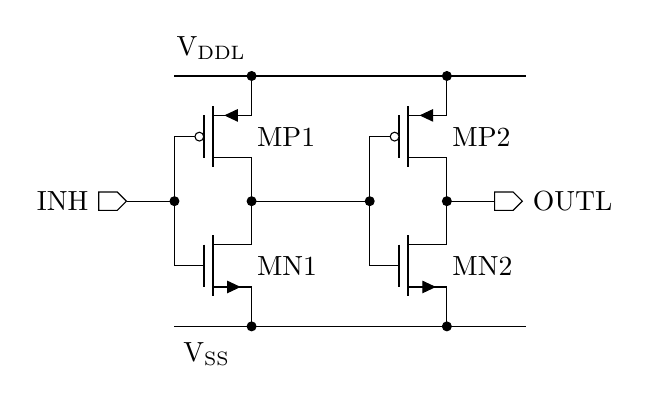
\begin{tikzpicture}[scale=1]
        \ctikzset{tripoles/mos style/arrows}
        \ctikzset{tripoles/pmos style/emptycircle}
        \ctikzset{logic ports=ieee}
        \draw (0,0)
        node[pmos, scale=1](pmos1){MP1}
        (pmos1.D) to [short] ++(0,-0.1) node[nmos, scale=1, anchor=D](nmos1){MN1}
        (pmos1.G) to (nmos1.G)
        ($(pmos1.G)!0.5!(nmos1.G)$) node[circ, scale=1]{} --++ (-0.6,0) node[signal, anchor=east, scale=1, draw](inh){} 
        (inh.west) node[anchor=east, scale=1]{INH}
        ($(pmos1.D)!0.5!(nmos1.D)$) node[circ, scale=1]{} --++(1.5,0) node[circ, scale=1]{}
        (nmos1.center) ++ (1.5,0) node[nmos, scale=1, anchor=G](nmos2){MN2}
        (nmos2.D) to [short] ++(0,0.1) node[pmos, scale=1, anchor=D](pmos2){MP2}
        (nmos2.G) to (pmos2.G)
        ($(pmos2.D)!0.5!(nmos2.D)$) node[circ, scale=1]{} --++ (0.6,0) node[signal, anchor=west, scale=1, draw](outl){}
        (outl.east) node[anchor=west, scale=1]{OUTL}
        (nmos1.G|-nmos1.S) -- (nmos1.S) node[circ, scale=1](vss){} -- (nmos2.S) node[circ, scale=1]{} --++ (1,0)
        (pmos1.G|-pmos1.S) -- (pmos1.S) node[circ, scale=1](vddl){} -- (pmos2.S) node[circ, scale=1]{} --++ (1,0)
	(vss) ++ (-0.15, -0.35) node[left, scale=1]{$\text{V}_\text{SS}$}
	(vddl) ++ (0.05, 0.35) node[left, scale=1]{$\text{V}_\text{DDL}$}
        ;
    \end{tikzpicture}
    \vspace{0.35cm}
    \label{HL_level_shifter}
    }
    \vfil
    \vspace{0.3cm}
    \subfloat[]{
    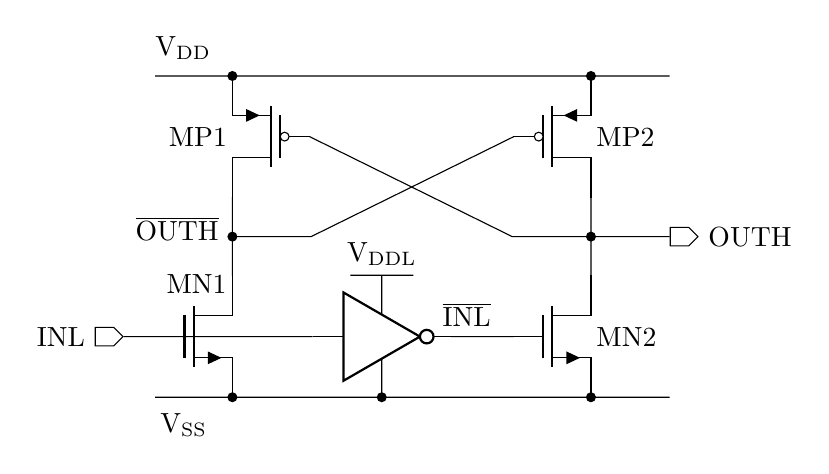
\begin{tikzpicture}[scale=1]
        \ctikzset{tripoles/mos style/arrows}
        \ctikzset{tripoles/pmos style/emptycircle}
        \ctikzset{logic ports=ieee}
        \draw 
        (0,0) node[nmos, anchor=G, scale=1](nmos1){} --++
        (2,0) node[ieeestd not port, anchor=in, scale=1](inv){}
        (nmos1.inner up) ++ (0.05,0.4) node[left, scale=1]{MN1}
        (inv.out) --++ (0.8,0) node[nmos, anchor=G, scale=1](nmos2){MN2} 
        (nmos2.D) --++ (0,0.5) node[circ, scale=1](out){} --++ (0,0.5) node[pmos, anchor=D, scale=1](pmos2){MP2}
        (nmos1.D) --++ (0,0.5) node[circ, scale=1](outb){} --++ (0,0.5) node[pmos, xscale=-1, anchor=D, scale=1](pmos1){\ctikzflipx{MP1}}
        (outb) --++ (1,0) -- (pmos2.G)
        (out) --++ (-1,0) -- (pmos1.G)
        (outb) ++ (-0.05,0.10) node[left, scale=1]{$\overline{\mbox{OUTH}}$}
        (out) --++ (1,0) node[signal, anchor=west, scale=1, draw](out_o){} 
        (out_o.east) node[anchor=west, scale=1]{OUTH}
        (nmos1.G) --++ (-0.4,0) node[signal, anchor=east, scale=1, draw](in){} 
        (in.west) node[anchor=east, scale=1]{INL} 
        (0,0|-nmos1.S) -- (nmos1.S) node[circ, scale=1](vss){} -- (inv.down|-nmos2.S) node[circ, scale=1]{} 
        (inv.down) |- (nmos2.S) node[circ, scale=1]{} --++ (1,0)
        (0,0|-pmos1.S) -- (pmos1.S) node[circ, scale=1](vddh){} -- (pmos2.S) node[circ, scale=1]{} --++ (1,0)
	(vss) ++ (-0.2, -0.35) node[left, scale=1]{$\text{V}_\text{SS}$}
	(vddh) ++ (-0.15, 0.35) node[left, scale=1]{$\text{V}_\text{DD}$}
	(inv.up) --++ (0,0.5) node[above, scale=1](vddl){$\text{V}_\text{DDL}$} ++ (-0.4,0) --++ (0.8,0)
        (inv.out) ++ (0.2,0) node[above, scale=1]{$\overline{\mbox{INL}}$}
        ;
    \end{tikzpicture}
    \label{LH_level_shifter}
    }
    \caption{Шема претварача (а) са високог на низак и (б) са ниског на висок напонски ниво \cite{Osaki:6198744}.}
    \label{Level_shifters}
\end{figure}

Како је напон напајања \DCO-а нижи од остатка система, на управљачке улазе \DCO-a постављени су претварачи са високог на низак напонски ниво \engl[HLLS]{High-Low Level Shifter}, док су на фазне излазе \DCO-a постављени претварачи са ниског на висок напонски ниво \engl[LHLS]{Low-High Level Shifter}. \figurename~\ref{Level_shifters} приказује шеме конвенционалних претварача напонског нивоа који су коришћени у претходно описаном систему. Као што се може видјети са Слике \ref{Level_shifters}, претварач са високог на низак напонски ниво није ништа друго до обичан бафер састављен од два инвертора чије напајање ће у коначној реализацији долазити од линије ниског напонског нивоа ($V_\text{DDL}$). Претварач са ниског на висок напонски ниво је нешто комплекснији и представља регенеративно логичко коло засновано на позитивној повратној спрези~\cite{Osaki:6198744} и састоји се од два унакрсно спрегнута PMOS транзистора, од NMOS транзистора и инвертора.\par
Претварачи напонских нивоа могу довести до сметњи у радном циклусу \engl{Duty Cycle}, поготово на излазу претварача са ниског на висок напонски ниво. Међутим, то се углавном може избјећи додатним баферовањем излаза \DCO-а тј. физичким уметањем одговарајућих бафера између фазног излаза \DCO-a и претварача напонског нивоа чиме се сигнал додатно исправља како би такав дошао на улаз претварача са ниског на висок напонски ниво.


\section{Имплементација и резултати симулација} \label{Implementation and results}
Дигитални \FLL\ описан у овом раду, имплементиран је коришћењем SystemVerilog језика за опис хардвера у 130~nm CMOS технологији. \DCO\ је имплементиран као независна компонента коришћењем библиотека стандардних ћелија. Читав дизајн \FLL-a заузима 33000\,\text\textmu m$^\text2$, од чега 13\,\% заузима \DCO. Референтни такт је 16\,MHz, док се такт \DCO-a подешава до 640\,MHz, при чему је резолуција учестаности око 2.8\,MHz у типичним условима рада. У симулацији под типичним условима рада, напон напајања управљачке логике \FLL-а ($V_\text{DD}$) је подешен на 1.2\,V, а самог \DCO-a ($V_\text{DDL}$) на 1.1\,V, и за њих је средња квадратна вриједност \engl[RMS]{Root Mean Square} потрошње струје 0.9\,mA и 2.185\,mA, респективно. Лејаут коначне верзије цјелокупног \FLL-а приказан је на Слици~\ref{layout_FLL}. 

\begin{figure}[!h]
	 \centering
	 \begin{tikzpicture}%[scale=0.21]
	 %\includegraphics[scale=0.21]{fig/layout_FLL.png}
	 % The image node
        \node[inner sep=0] (layout_FLL) { \includegraphics[scale=0.37]{slike/layout_FLL.png} };
        \draw[<->] (-7.7,-2.25) -- (-7.7,2.25) node[midway, left=0.2, above=0.05, rotate=90] {\footnotesize 100\,\textmu m};
        \draw[<->] (-7.45,-2.6) -- (7.45,-2.6) node[midway, right=0.1, below=0.02] {\footnotesize 330\,\textmu m};
        \end{tikzpicture}	
	\caption{Лејаут дигиталног \FLL-а, са \DCO-ом у доњем десном углу.}
	\label{layout_FLL}
\end{figure}


\subsection{Симулација рада фреквенцијски затворене петље}
Симулација рада \FLL-a у оба управљачка режима приказана је на Слици~\ref{sim_FLL}. Са приказаних графика се може видјети да се у оба управљачка режима достиже стабилно закључавање \FLL-a са излазном фреквенцијом веома блиској траженој фреквенцији, при чему грешка може бити у опсегу просјечне вриједности резолуције \DCO-а (испод 3\,MHz). Међутим, иако се у оба режима исправно достиже жељена фреквенција, између њих постоји разлика у брзини достизања исте. Тако, у \PID\ режиму (\P=15, \I=15, \D=0), закључавање се одвија много брже, и то за 1.83\,\textmu s, док је, поређења ради, за закључавање у bang-bang режиму потребно 13.13\,\textmu s.

\begin{figure}[!ht]
    \centering
    \subfloat[]{
	    % FLL control simulation - PID mode
%\begin{figure}[h]%[ht]
%    \vspace{-0.6cm} % added to avoid empty space above the figure
    \begin{tikzpicture}[scale=1, every node/.style={scale=1}]
	        \pgfplotsset{%
                    width=14cm,
                    height=10cm
                }
       % Wave dimension setup
		\def \waveDigHeight {1.0}
		\def \waveAnaHeight {3.0}
		\def \waveSpacing   {1.0}
		\def \waveOffset    {0.2}
		% Group plot
		\begin{groupplot}
			[xlabel={\footnotesize Time [\textmu s]},
			 axis line style={draw=none}, % remove axis lines and arrows
			 xtick style={draw=none}, % remove tick dash
			 ytick style={draw=none}, % remove tick dash
			 xticklabel style = {font=\footnotesize},
			 ymin=0, ymax=22, % NUM_WAVES*WAVE_HEIGHT+(NUM_WAVES+1)*WAVE_SPACING
			 xmin=0, xmax=3.0,
			 yticklabel style={xshift=0.2em} % move labels closer to axis
			]			
			% Wave position and max/min value setup
			%\def \waveDCOclkY    {2.5}
			%\def \waveFllFreqY   {\waveDCOclkY+\waveDigHeight*0.5+\waveSpacing+\waveAnaHeight*0.5}
			\def \waveFllLockY   {1.5}
			\def \waveFllFreqY   {\waveFllLockY+\waveAnaHeight*0.5+\waveSpacing+\waveDigHeight*0.5}
			\def \waveFllFreqMax {650}
			\def \waveFllFreqMin {0}
			\def \waveDCOcodeY   {\waveFllFreqY+\waveAnaHeight+\waveSpacing}
			\def \waveDCOcodeMax {255}
			\def \waveDCOcodeY   {\waveFllFreqY+\waveAnaHeight+\waveSpacing}
			\def \waveDCOcodeMax {255}
			\def \waveDCOcntY    {\waveDCOcodeY+\waveAnaHeight+\waveSpacing}
			\def \waveDCOcntMax  {25}
			\def \waveClkDivY    {\waveDCOcntY+\waveAnaHeight*0.5+\waveSpacing+\waveDigHeight*0.5}
			\def \waveRstnY      {\waveClkDivY+\waveDigHeight+\waveSpacing}
			% Draw rectangle round group plot
			\draw (0,0) rectangle (30.1em,17.6em);
			% Set up group plot
			\nextgroupplot[ylabel={}, 
			               ytick={\waveFllLockY, \waveFllLockY-0.5*\waveDigHeight+\waveOffset, \waveFllLockY+0.5*\waveDigHeight-\waveOffset, % FLL lock
			                      \waveFllFreqY, \waveFllFreqY-0.5*\waveAnaHeight+\waveOffset, \waveFllFreqY+0.5*\waveAnaHeight-\waveOffset, % FLL frequency
			                      \waveDCOcodeY, \waveDCOcodeY-0.5*\waveAnaHeight+\waveOffset, \waveDCOcodeY+0.5*\waveAnaHeight-\waveOffset, % DCO control code
			                      \waveDCOcntY,   \waveDCOcntY-0.5*\waveAnaHeight+\waveOffset,  \waveDCOcntY+0.5*\waveAnaHeight-\waveOffset, % DCO counter
			                      \waveClkDivY,   \waveClkDivY-0.5*\waveDigHeight+\waveOffset,  \waveClkDivY+0.5*\waveDigHeight-\waveOffset, % Clock
			                      \waveRstnY,       \waveRstnY-0.5*\waveDigHeight+\waveOffset,    \waveRstnY+0.5*\waveDigHeight-\waveOffset  % Reset
			                     },
			               extra y ticks={\waveFllLockY-0.5*\waveDigHeight, \waveFllLockY+0.5*\waveDigHeight, % FLL lock
                			              \waveFllFreqY-0.5*\waveAnaHeight, \waveFllFreqY+0.5*\waveAnaHeight, % FLL frequency
			                              \waveDCOcodeY-0.5*\waveAnaHeight, \waveDCOcodeY+0.5*\waveAnaHeight, % DCO control code
			                               \waveDCOcntY-0.5*\waveAnaHeight,  \waveDCOcntY+0.5*\waveAnaHeight, % DCO counter
			                               \waveClkDivY-0.5*\waveDigHeight,  \waveClkDivY+0.5*\waveDigHeight, % Clock
			                                 \waveRstnY-0.5*\waveDigHeight,    \waveRstnY+0.5*\waveDigHeight  % Reset
			                             },
			               extra tick style={grid=major, color=lightgray, dotted},        
			               extra y tick labels={},       
			               yticklabels={\textcolor{\DCOColor}{\footnotesize \framebox{FLL lock} \hspace{5pt}},
			                            \textcolor{\DCOColor}{\scriptsize 0},
			                            \textcolor{\DCOColor}{\scriptsize 1},
			                            \textcolor{\DCOColor}{\footnotesize \framebox{FLL freq} \hspace{5pt}},
			                            \textcolor{\DCOColor}{\scriptsize \waveFllFreqMin},
			                            \textcolor{\DCOColor}{\scriptsize \waveFllFreqMax},
			                            \textcolor{\PIDctrlColor}{\footnotesize \framebox{DCO code} \hspace{5pt}},
			                            \textcolor{\PIDctrlColor}{\scriptsize 0},
			                            \textcolor{\PIDctrlColor}{\scriptsize \waveDCOcodeMax},
			                            \textcolor{\CtrlPreprocColor}{\footnotesize \framebox{DCO cnt} \hspace{5pt}},
			                            \textcolor{\CtrlPreprocColor}{\scriptsize 0},
			                            \textcolor{\CtrlPreprocColor}{\scriptsize \waveDCOcntMax },
			                            \textcolor{\ClkDivColor}{\footnotesize \framebox{Clock} \hspace{5pt}},
			                            \textcolor{\ClkDivColor}{\scriptsize 0},
			                            \textcolor{\ClkDivColor}{\scriptsize 1},
			                            \textcolor{\RstnColor}{\footnotesize \framebox{Reset} \hspace{5pt}},
			                            \textcolor{\RstnColor}{\scriptsize 0},
			                            \textcolor{\RstnColor}{\scriptsize 1}                                                      
			                           }
			              ]
			% Reset signal			
			\addplot [ line width=0.4pt, \RstnColor,
			           shift={(axis direction cs:0,\waveRstnY-0.5*\waveDigHeight)}
			         ] table [x index=0, 
			                  y expr=\thisrowno{1}, 
			                  col sep=comma
			                 ] {wav/pid/fll_tb.u_fll.rst_ni.csv};
			% Clock signal
			\addplot [ line width=0.4pt, \ClkDivColor ,
			           shift={(axis direction cs:0,\waveClkDivY-0.5*\waveDigHeight)}
			         ] table [x index=0, 
			                  y expr=\thisrowno{1}, 
			                  col sep=comma
			                 ] {wav/pid/fll_tb.u_fll.clk_ref_div2.csv};
			% DCO counter sampled & synchronized			
			\addplot [ line width=0.4pt, \CtrlPreprocColor,
			           shift={(axis direction cs:0,\waveDCOcntY-0.5*\waveAnaHeight)}
			         ] table [x index=0, 
			                  y expr=\thisrowno{1}*\waveAnaHeight/\waveDCOcntMax, 
			                  col sep=comma
			                 ] {wav/pid/fll_tb.u_fll.cnt_dco_q.csv};
			% DCO code
			\addplot [ line width=0.4pt, \PIDctrlColor, 
			           shift={(axis direction cs:0,\waveDCOcodeY-0.5*\waveAnaHeight)}
			         ] table [x index=0, 
			                  y expr=\thisrowno{1}*\waveAnaHeight/\waveDCOcodeMax, 
			                  col sep=comma
			                 ] {wav/pid/fll_tb.u_fll.u_dco.code.csv};                 
            % FLL Frequency        
			\addplot [ line width=0.4pt, \DCOColor,
			           shift={(axis direction cs:0,\waveFllFreqY-0.5*\waveAnaHeight)}
			         ] table [x index=0, 
			                  y expr=\thisrowno{1}*\waveAnaHeight/\waveFllFreqMax, 
			                  col sep=comma
			                 ] {wav/pid/fll_tb.u_fll.u_dco.dco_freq_MHz.csv};    
            % FLL Lock        
			\addplot [ line width=0.4pt, \DCOColor,
			           shift={(axis direction cs:0,\waveFllLockY-0.5*\waveDigHeight)}
			         ] table [x index=0, 
			                  y expr=\thisrowno{1}, 
			                  col sep=comma
			                 ] {wav/pid/fll_tb.u_fll.lock_o.csv};               
		\end{groupplot}
		% Mark lock time
		\draw[<->]             (2.7,7.55) -- (10.4,7.55) node[midway, above=0.005] {\footnotesize Вријеме закључавања \FLL-a у \PID\ режиму: 1.825\,\textmu s};
		\draw[-, gray, dashed] (2.69,1.4) -- (2.69,7.7);
		\draw[-, gray, dashed] (10.41,0.77) -- (10.41,7.7);
    \end{tikzpicture}
%	\caption{FLL control simulation: PID mode, locking time of 1.8\,\textmu s.}
%	\label{sim_PID}    
%\end{figure}

    }
    %\hfil
    \vspace{0.2cm}
    \subfloat[]{		
	    \hspace{-0.2cm}
	    % FLL control simulation - bang-bang mode
%\begin{figure}[h]%[ht]
    \begin{tikzpicture}[scale=0.9, every node/.style={scale=1}]
	        \pgfplotsset{%
                    width=14cm,
                    height=10.5cm
                }
       % Wave dimension setup
		\def \waveDigHeight {1.0}
		\def \waveAnaHeight {3.0}
		\def \waveSpacing   {1.0}
		\def \waveOffset    {0.2}
		% Group plot
		\begin{groupplot}
			[xlabel={\footnotesize Вријеме [\textmu s]},
			 axis line style={draw=none}, % remove axis lines and arrows
			 xtick style={draw=none}, % remove tick dash
			 ytick style={draw=none}, % remove tick dash
			 xticklabel style = {font=\footnotesize},
			 ymin=0, ymax=22, % NUM_WAVES*WAVE_HEIGHT+(NUM_WAVES+1)*WAVE_SPACING
			 xmin=0, xmax=15.0,
			 yticklabel style={xshift=0.2em}, % move labels closer to axis
			 xtick={0,1,...,15}
			]			
			% Wave position and max/min value setup
			%\def \waveDCOclkY    {2.5}
			%\def \waveFllFreqY   {\waveDCOclkY+\waveDigHeight*0.5+\waveSpacing+\waveAnaHeight*0.5}
			\def \waveFllLockY   {1.5}
			\def \waveFllFreqY   {\waveFllLockY+\waveAnaHeight*0.5+\waveSpacing+\waveDigHeight*0.5}
			\def \waveFllFreqMax {650}
			\def \waveFllFreqMin {0}
			\def \waveDCOcodeY   {\waveFllFreqY+\waveAnaHeight+\waveSpacing}
			\def \waveDCOcodeMax {255}
			\def \waveDCOcodeY   {\waveFllFreqY+\waveAnaHeight+\waveSpacing}

			\def \waveBBupdnY  {\waveDCOcodeY+\waveAnaHeight*0.5+\waveSpacing+\waveDigHeight*0.5}
			\def \waveBBenY    {\waveBBupdnY+\waveDigHeight+\waveSpacing}

			\def \waveDCOcntY    {\waveBBenY+\waveAnaHeight*0.5+\waveSpacing+\waveDigHeight*0.5}
			\def \waveDCOcntMax  {25}
			
			\def \waveClkDivY    {\waveDCOcntY+\waveAnaHeight*0.5+\waveSpacing+\waveDigHeight*0.5}
			\def \waveRstnY      {\waveClkDivY+\waveDigHeight+\waveSpacing}
			% Draw rectangle round group plot
			\draw (0,0) rectangle (30.1em,22.5em); % [line width=0.8pt]
			% Set up group plot
			\nextgroupplot[ylabel={}, 
			               ytick={\waveFllLockY, \waveFllLockY-0.5*\waveDigHeight+\waveOffset, \waveFllLockY+0.5*\waveDigHeight-\waveOffset, % FLL frequency
			                      \waveFllFreqY, \waveFllFreqY-0.5*\waveAnaHeight+\waveOffset, \waveFllFreqY+0.5*\waveAnaHeight-\waveOffset, % FLL frequency
			                      \waveDCOcodeY, \waveDCOcodeY-0.5*\waveAnaHeight+\waveOffset, \waveDCOcodeY+0.5*\waveAnaHeight-\waveOffset, % DCO control code
			                      \waveBBupdnY,   \waveBBupdnY-0.5*\waveDigHeight+\waveOffset,  \waveBBupdnY+0.5*\waveDigHeight-\waveOffset, % Clock
   			                      \waveBBenY,   \waveBBenY-0.5*\waveDigHeight+\waveOffset,  \waveBBenY+0.5*\waveDigHeight-\waveOffset, % Clock			                      
			                      \waveDCOcntY,   \waveDCOcntY-0.5*\waveAnaHeight+\waveOffset,  \waveDCOcntY+0.5*\waveAnaHeight-\waveOffset, % DCO counter
			                      \waveClkDivY,   \waveClkDivY-0.5*\waveDigHeight+\waveOffset,  \waveClkDivY+0.5*\waveDigHeight-\waveOffset, % Clock
			                      \waveRstnY,       \waveRstnY-0.5*\waveDigHeight+\waveOffset,    \waveRstnY+0.5*\waveDigHeight-\waveOffset  % Reset
			                     },
			               extra y ticks={\waveFllLockY-0.5*\waveDigHeight, \waveFllLockY+0.5*\waveDigHeight, % FLL lock
                     		              \waveFllFreqY-0.5*\waveAnaHeight, \waveFllFreqY+0.5*\waveAnaHeight, % FLL frequency
			                              \waveDCOcodeY-0.5*\waveAnaHeight, \waveDCOcodeY+0.5*\waveAnaHeight, % DCO control code
                                          \waveBBupdnY-0.5*\waveDigHeight,  \waveBBupdnY+0.5*\waveDigHeight, % Clock
                                          \waveBBenY-0.5*\waveDigHeight,  \waveBBenY+0.5*\waveDigHeight, % Clock			                              
			                               \waveDCOcntY-0.5*\waveAnaHeight,  \waveDCOcntY+0.5*\waveAnaHeight, % DCO counter
			                               \waveClkDivY-0.5*\waveDigHeight,  \waveClkDivY+0.5*\waveDigHeight, % Clock
			                                 \waveRstnY-0.5*\waveDigHeight,    \waveRstnY+0.5*\waveDigHeight  % Reset
			                             },
			               extra tick style={grid=major, color=lightgray, dotted},        
			               extra y tick labels={},       
			               yticklabels={\textcolor{\DCOColor}{\footnotesize \framebox{FLL lock} \hspace{5pt}},
			                            \textcolor{\DCOColor}{\scriptsize 0},
			                            \textcolor{\DCOColor}{\scriptsize 1},
			                            \textcolor{\DCOColor}{\footnotesize \framebox{FLL freq} \hspace{5pt}},
			                            \textcolor{\DCOColor}{\scriptsize \waveFllFreqMin},
			                            \textcolor{\DCOColor}{\scriptsize \waveFllFreqMax},
			                            \textcolor{\BBctrlColor}{\footnotesize \framebox{DCO code} \hspace{5pt}},
			                            \textcolor{\BBctrlColor}{\scriptsize 0},
			                            \textcolor{\BBctrlColor}{\scriptsize \waveDCOcodeMax},
			                            \textcolor{\BBctrlColor}{\footnotesize \framebox{BB updn} \hspace{5pt}},
			                            \textcolor{\BBctrlColor}{\scriptsize 0},
			                            \textcolor{\BBctrlColor}{\scriptsize 1},
			                            \textcolor{\BBctrlColor}{\footnotesize \framebox{BB en} \hspace{5pt}},
			                            \textcolor{\BBctrlColor}{\scriptsize 0},
			                            \textcolor{\BBctrlColor}{\scriptsize 1},			                            			                            
			                            \textcolor{\CtrlPreprocColor}{\footnotesize \framebox{DCO cnt} \hspace{5pt}},
			                            \textcolor{\CtrlPreprocColor}{\scriptsize 0},
			                            \textcolor{\CtrlPreprocColor}{\scriptsize \waveDCOcntMax },
			                            \textcolor{\ClkDivColor}{\footnotesize \framebox{Clock} \hspace{5pt}},
			                            \textcolor{\ClkDivColor}{\scriptsize 0},
			                            \textcolor{\ClkDivColor}{\scriptsize 1},
			                            \textcolor{\RstnColor}{\footnotesize \framebox{Reset} \hspace{5pt}},
			                            \textcolor{\RstnColor}{\scriptsize 0},
			                            \textcolor{\RstnColor}{\scriptsize 1}                                                      
			                           }
			              ]
			% Reset signal			
			\addplot [ line width=0.5pt, \RstnColor,
			           shift={(axis direction cs:0,\waveRstnY-0.5*\waveDigHeight)}
			         ] table [x index=0, 
			                  y expr=\thisrowno{1}, 
			                  col sep=comma
			                 ] {wav/bb/fll_tb.u_fll.rst_ni.csv};
			% Clock signal
			\addplot [ line width=0.2pt, \ClkDivColor ,
			           shift={(axis direction cs:0,\waveClkDivY-0.5*\waveDigHeight)}
			         ] table [x index=0, 
			                  y expr=\thisrowno{1}, 
			                  col sep=comma
			                 ] {wav/bb/fll_tb.u_fll.clk_ref_div2.csv};
			% DCO counter sampled & synchronized			
			\addplot [ line width=0.5pt, \CtrlPreprocColor,
			           shift={(axis direction cs:0,\waveDCOcntY-0.5*\waveAnaHeight)}
			         ] table [x index=0, 
			                  y expr=\thisrowno{1}*\waveAnaHeight/\waveDCOcntMax, 
			                  col sep=comma
			                 ] {wav/bb/fll_tb.u_fll.cnt_dco_q.csv};
			% CNT enable signal
			\addplot [ line width=0.5pt, \BBctrlColor ,
			           shift={(axis direction cs:0,\waveBBenY-0.5*\waveDigHeight)}
			         ] table [x index=0, 
			                  y expr=\thisrowno{1}, 
			                  col sep=comma
			                 ] {wav/bb/fll_tb.u_fll.u_cnt_ref.en_i.csv};
			% CNT up down signal
			\addplot [ line width=0.5pt, \BBctrlColor ,
			           shift={(axis direction cs:0,\waveBBupdnY-0.5*\waveDigHeight)}
			         ] table [x index=0, 
			                  y expr=\thisrowno{1}, 
			                  col sep=comma
			                 ] {wav/bb/fll_tb.u_fll.u_cnt_ref.up_down_i.csv};			                 			                 
   			% DCO code
			\addplot [ line width=0.5pt, \BBctrlColor, 
			           shift={(axis direction cs:0,\waveDCOcodeY-0.5*\waveAnaHeight)}
			         ] table [x index=0, 
			                  y expr=\thisrowno{1}*\waveAnaHeight/\waveDCOcodeMax, 
			                  col sep=comma
			                 ] {wav/bb/fll_tb.u_fll.u_dco.code.csv};                 
            % FLL Frequency        
			\addplot [ line width=0.5pt, \DCOColor,
			           shift={(axis direction cs:0,\waveFllFreqY-0.5*\waveAnaHeight)}
			         ] table [x index=0, 
			                  y expr=\thisrowno{1}*\waveAnaHeight/\waveFllFreqMax, 
			                  col sep=comma
			                 ] {wav/bb/fll_tb.u_fll.u_dco.dco_freq_MHz.csv};  
            % FLL Lock        
			\addplot [ line width=0.5pt, \DCOColor,
			           shift={(axis direction cs:0,\waveFllLockY-0.5*\waveDigHeight)}
			         ] table [x index=0, 
			                  y expr=\thisrowno{1}, 
			                  col sep=comma
			                 ] {wav/bb/fll_tb.u_fll.lock_o.csv}; 			                                
		\end{groupplot}
		% Mark lock time
		\draw[<->]             (0.05,9.6) -- (11.04,9.6) node[midway, above] {\footnotesize Вријеме закључавања \FLL-а у bang-bang режиму: 13.124\,\textmu s};
		\draw[-, gray, dashed] (0.00,9.4) -- (0.00,9.8);
		\draw[-, gray, dashed] (11.09,0.8) -- (11.09,9.8);
    \end{tikzpicture}
%	\caption{FLL control simulation: bang-bang mode, locking time of 13\,\textmu s.}	
%	\label{sim_BB}    
%\end{figure}

    }	
    \caption {Симулација \FLL-а у (а) PID режиму и (б) bang-bang режиму.} % , lock time 1.8\,\textmu s lock time 13.3\,\textmu s
    \label{sim_FLL}
\end{figure}

\subsection{\PVT\ зависност дигитално контролисаног осцилатора}
Да би се одредило понашање \DCO-a у реалним условима, потребно је провјерити понашање \DCO-а при промјени процесних углова, напона напајања и температуре, односно провјерити различите \PVT\ случајеве. У оквиру овог рада симулирано је понашање у три различита \PVT\ случаја:
\begin{enumerate}
	\item Најгори (најспорији) случај (slow-slow процесни угао, $V_\text{DD}$=1.1\,V, $V_\text{DDL}$=1\,V, 125\,$^{\circ}$C)
	\item Типичан случај (typical-typical процесни угао, $V_\text{DD}$=1.2\,V, $V_\text{DDL}$=1.1\,V, 40\,$^{\circ}$C)
	\item Најбољи (најбржи) случај (fast-fast процесни угао, $V_\text{DD}$=1.3\,V, $V_\text{DDL}$=1.2\,V, \\ -40\,$^{\circ}$C)
\end{enumerate}
Да би се значајно смањило вријеме потребно за добијање резултата из симулација након екстракције лејаута, и то без губљења прецизности добијених резултата, симулације \DCO-a су извршене на нивоу појединачно екстракованих ћелија \DCO-a и екстракованих претварача напонског нивоа, са додатним паразитним кондензатором на свакој фази \DCO-a. Улога тих кондензатора је да надомјесте паразитне капацитивности које се јављају у потпуно екстракованом лејауту \DCO-a због међусобно повезаних ћелија, а које нису аутоматски урачунате ако се симулације врше на нивоу појединачно екстракованих компоненти \DCO-a, као што је то овде случај. Вриједност капацитивности додатог кондензатора прорачуната је на основу извјештаја генерисаног из екстракције на нивоу читавог дизајна. \par 
\figurename~\ref{DCO_worst_typical_best} приказује зависност фреквенције \DCO-a и фреквенцијског корака тј. резолуције фреквенције ($K_\text{DCO}$) од броја укључених тростатичких инвертора (тј. од управљачке ријечи \DCO-a), за најгори, типични и најбољи \PVT\ случај. 
\begin{figure*}[!ht]
    \centering

    \def \SSLineStyle {solid}
    \def \TTLineStyle {dashed}
    \def \FFLineStyle {dotted}
    
    \begin{tikzpicture}[scale=1]
    \pgfplotsset{%
        width=13cm,
        height=8cm
    }
    
    \definecolor{darkgray176}{RGB}{176,176,176}
    \definecolor{darkorange25512714}{RGB}{255,127,14}
    \definecolor{forestgreen4416044}{RGB}{44,160,44}
    \definecolor{steelblue31119180}{RGB}{31,119,180}
    
    \begin{axis}[
    tick align=outside,
    tick pos=left,
    x grid style={darkgray176},
    xlabel={Број укључених тростатичких инвертора \\ \vspace{0.2cm} \scriptsize (а)},
    xmajorgrids,
    xmin=0, xmax=255,
    xtick style={color=black},
    y grid style={darkgray176},
    ylabel={Учестаност осциловања [MHz]},
    ymajorgrids,
    ymin=0, ymax=1205.20885915,
    ytick style={color=black},
    %
    %ytick={0,0.2,...,1.2},
    xlabel style={align=center,text width=8cm},
    line width = 1pt,
    x axis line style = {line width=0.2pt},
    y axis line style = {line width=0.2pt},
    x grid style = {line width=0.2pt},
    y grid style = {line width=0.2pt},
    legend style={legend image post style={scale=0.82}, cells={anchor=west}, at={(0.648,1)}, font=\scriptsize, line width=0.5pt, legend reversed=true},
    tick label style={font=\footnotesize},
    label style={font=\footnotesize}
    ]
    \addplot [steelblue31119180, densely dashdotted]
    table {%
    0 27.191722
    1 28.683692
    2 30.309022
    3 32.11723
    4 34.134108
    5 36.358849
    6 37.927839
    7 39.606522
    8 41.430148
    9 43.414902
    10 45.554272
    11 47.174534
    12 48.887188
    13 50.720641
    14 52.68493
    15 54.771083
    16 56.427611
    17 58.164409
    18 60.0042
    19 61.954452
    20 64.007413
    21 65.690771
    22 67.44532
    23 69.289918
    24 71.229922
    25 73.257242
    26 74.962749
    27 76.730844
    28 78.579089
    29 80.511547
    30 82.517721
    31 84.240189
    32 86.019275
    33 87.87023
    34 89.796495
    35 91.79011
    36 93.526205
    37 95.314322
    38 97.167628
    39 99.088945
    40 101.070794
    41 102.818292
    42 104.613825
    43 106.469028
    44 108.386206
    45 110.354897
    46 112.11219
    47 113.913779
    48 115.770365
    49 117.683955
    50 119.647843
    51 121.413426
    52 123.220223
    53 125.078063
    54 126.988684
    55 128.945622
    56 130.718323
    57 132.529561
    58 134.388405
    59 136.296348
    60 138.242793
    61 140.021384
    62 141.836325
    63 143.695732
    64 145.601154
    65 147.546651
    66 149.330662
    67 151.14897
    68 153.008844
    69 154.912044
    70 156.852808
    71 158.64145
    72 160.462351
    73 162.323016
    74 164.224186
    75 166.154293
    76 167.947066
    77 169.76998
    78 171.630616
    79 173.529556
    80 175.4617
    81 177.257776
    82 179.082802
    83 180.943476
    84 182.840426
    85 184.768859
    86 186.567966
    87 188.394574
    88 190.255106
    89 192.150201
    90 194.067708
    91 195.869229
    92 197.696975
    93 199.55706
    94 201.450152
    95 203.37153
    96 205.175238
    97 207.004077
    98 208.863785
    99 210.754961
    100 212.673127
    101 214.478698
    102 216.308353
    103 218.167614
    104 220.056974
    105 221.963372
    106 223.770465
    107 225.600614
    108 227.459159
    109 229.346606
    110 231.25865
    111 233.067029
    112 234.897632
    113 236.755409
    114 238.641014
    115 240.550167
    116 242.35969
    117 244.190488
    118 246.047606
    119 247.931217
    120 249.827601
    121 251.637704
    122 253.468492
    123 255.324449
    124 257.206159
    125 259.109619
    126 260.92044
    127 262.751138
    128 264.606284
    129 266.48596
    130 268.386715
    131 270.198051
    132 272.028506
    133 273.882537
    134 275.760405
    135 277.647267
    136 279.458722
    137 281.288715
    138 283.141425
    139 285.01718
    140 286.91245
    141 288.724039
    142 290.553655
    143 292.405095
    144 294.279123
    145 296.171641
    146 297.983143
    147 299.811979
    148 301.662181
    149 303.53398
    150 305.411572
    151 307.222799
    152 309.050839
    153 310.899508
    154 312.769166
    155 314.656416
    156 316.467377
    157 318.294549
    158 320.141819
    159 322.009433
    160 323.894166
    161 325.704609
    162 327.530916
    163 329.376723
    164 331.242232
    165 333.110937
    166 334.920747
    167 336.745866
    168 338.589953
    169 340.453576
    170 342.332475
    171 344.141644
    172 345.965705
    173 347.808323
    174 349.669451
    175 351.545956
    176 353.354358
    177 355.177354
    178 357.018215
    179 358.877281
    180 360.736895
    181 362.544478
    182 364.365929
    183 366.205254
    184 368.061598
    185 369.932965
    186 371.73953
    187 373.559829
    188 375.397301
    189 377.251696
    190 379.120535
    191 380.926131
    192 382.745413
    193 384.580603
    194 386.432973
    195 388.283774
    196 390.088104
    197 391.905518
    198 393.739259
    199 395.58889
    200 397.452384
    201 399.255663
    202 401.071697
    203 402.903377
    204 404.750972
    205 406.611846
    206 408.4139
    207 410.228344
    208 412.058177
    209 413.903564
    210 415.745685
    211 417.546058
    212 419.358654
    213 421.186324
    214 423.02925
    215 424.884318
    216 426.683404
    217 428.494383
    218 430.319965
    219 432.160432
    220 434.013173
    221 435.810455
    222 437.619585
    223 439.443077
    224 441.281017
    225 443.114408
    226 444.910071
    227 446.717308
    228 448.538548
    229 450.373892
    230 452.220852
    231 454.015125
    232 455.820523
    233 457.639547
    234 459.472498
    235 461.317092
    236 463.109712
    237 464.913431
    238 466.729888
    239 468.560691
    240 470.384824
    241 472.175653
    242 473.977148
    243 475.791426
    244 477.619333
    245 479.457898
    246 481.246909
    247 483.04653
    248 484.858643
    249 486.684185
    250 488.519905
    251 490.307353
    252 492.10481
    253 493.914574
    254 495.73728
    255 497.551513
    };
    \addlegendentry{slow-slow; T=125\,\textdegree C; $\text{V}_\text{\scalebox{.8}{DD}}$=1,1\,V; $\text{V}_\text{\scalebox{.8}{DDL}}$=1,0\,V}
    \addplot [darkorange25512714, solid]
    table {%
    0 41.980536
    1 44.285759
    2 46.800092
    3 49.592026
    4 52.695336
    5 56.12135
    6 58.543564
    7 61.137623
    8 63.951508
    9 67.005382
    10 70.29997
    11 72.799263
    12 75.444178
    13 78.270747
    14 81.293314
    15 84.504829
    16 87.059249
    17 89.739325
    18 92.574521
    19 95.57499
    20 98.733878
    21 101.329367
    22 104.035538
    23 106.877014
    24 109.861507
    25 112.982165
    26 115.608572
    27 118.335019
    28 121.181051
    29 124.153221
    30 127.239692
    31 129.892276
    32 132.634172
    33 135.483782
    34 138.446018
    35 141.512996
    36 144.186168
    37 146.941013
    38 149.793237
    39 152.747491
    40 155.795909
    41 158.486062
    42 161.251166
    43 164.10585
    44 167.05339
    45 170.080595
    46 172.785184
    47 175.55891
    48 178.415208
    49 181.35721
    50 184.376559
    51 187.093413
    52 189.874405
    53 192.732082
    54 195.668856
    55 198.677261
    56 201.404631
    57 204.191734
    58 207.050398
    59 209.98275
    60 212.973611
    61 215.709758
    62 218.501786
    63 221.360914
    64 224.288858
    65 227.278719
    66 230.022541
    67 232.818928
    68 235.678449
    69 238.602591
    70 241.584825
    71 244.334972
    72 247.135499
    73 249.99504
    74 252.915539
    75 255.880817
    76 258.636539
    77 261.439741
    78 264.299201
    79 267.21614
    80 270.184578
    81 272.94528
    82 275.750967
    83 278.610066
    84 281.523599
    85 284.48575
    86 287.250524
    87 290.058151
    88 292.91649
    89 295.826729
    90 298.771004
    91 301.539045
    92 304.347929
    93 307.205248
    94 310.111964
    95 313.062538
    96 315.833489
    97 318.643503
    98 321.499889
    99 324.403309
    100 327.348559
    101 330.122078
    102 332.933015
    103 335.788259
    104 338.688665
    105 341.614783
    106 344.390453
    107 347.201468
    108 350.055272
    109 352.95225
    110 355.887401
    111 358.664492
    112 361.475893
    113 364.32829
    114 367.222055
    115 370.152446
    116 372.93075
    117 375.742182
    118 378.592947
    119 381.483675
    120 384.393263
    121 387.172372
    122 389.983251
    123 392.832276
    124 395.719279
    125 398.640225
    126 401.41992
    127 404.23046
    128 407.077446
    129 409.961375
    130 412.877864
    131 415.658001
    132 418.467849
    133 421.312735
    134 424.193518
    135 427.087857
    136 429.867772
    137 432.676253
    138 435.518955
    139 438.396133
    140 441.303408
    141 444.083206
    142 446.89066
    143 449.731049
    144 452.604822
    145 455.507758
    146 458.287216
    147 461.093308
    148 463.931712
    149 466.802026
    150 469.681241
    151 472.459776
    152 475.264275
    153 478.099818
    154 480.966521
    155 483.860552
    156 486.638306
    157 489.441426
    158 492.274394
    159 495.137573
    160 498.027247
    161 500.804132
    162 503.60537
    163 506.435672
    164 509.295468
    165 512.160319
    166 514.936125
    167 517.73455
    168 520.561892
    169 523.418103
    170 526.298719
    171 529.072612
    172 531.869579
    173 534.694142
    174 537.546609
    175 540.423189
    176 543.195685
    177 545.990542
    178 548.812286
    179 551.661216
    180 554.511843
    181 557.282498
    182 560.074963
    183 562.893713
    184 565.738981
    185 568.606284
    186 571.375236
    187 574.16546
    188 576.980994
    189 579.822453
    190 582.68588
    191 585.453374
    192 588.241436
    193 591.054035
    194 593.891796
    195 596.728417
    196 599.49358
    197 602.278669
    198 605.087983
    199 607.921725
    200 610.776491
    201 613.539269
    202 616.32164
    203 619.127712
    204 621.957577
    205 624.80784
    206 627.568277
    207 630.347927
    208 633.150629
    209 635.976506
    210 638.799
    211 641.556885
    212 644.333791
    213 647.132365
    214 649.954423
    215 652.795215
    216 655.550541
    217 658.324041
    218 661.119534
    219 663.937371
    220 666.774007
    221 669.527029
    222 672.297472
    223 675.089495
    224 677.903431
    225 680.711739
    226 683.461687
    227 686.228739
    228 689.016947
    229 691.826443
    230 694.653712
    231 697.40069
    232 700.165155
    233 702.949415
    234 705.754892
    235 708.57774
    236 711.322079
    237 714.083332
    238 716.864109
    239 719.665606
    240 722.459816
    241 725.20045
    242 727.957823
    243 730.734957
    244 733.531914
    245 736.34547
    246 739.084153
    247 741.837736
    248 744.610922
    249 747.404152
    250 750.212875
    251 752.94865
    252 755.698776
    253 758.469037
    254 761.257793
    255 764.034889
    };
    \addlegendentry{typical-typical; T=40\,\textdegree C; $\text{V}_\text{\scalebox{.8}{DD}}$=1,2\,V; $\text{V}_\text{\scalebox{.8}{DDL}}$=1,1\,V}
    \addplot [forestgreen4416044, densely dotted]
    table {%
    0 63.313495
    1 66.788901
    2 70.585845
    3 74.793272
    4 79.453051
    5 84.606318
    6 88.254323
    7 92.168267
    8 96.404905
    9 100.991931
    10 105.947313
    11 109.709158
    12 113.695569
    13 117.95091
    14 122.488761
    15 127.316862
    16 131.160345
    17 135.197792
    18 139.462686
    19 143.968235
    20 148.716378
    21 152.620132
    22 156.694628
    23 160.967364
    24 165.44824
    25 170.13638
    26 174.086846
    27 178.189442
    28 182.467808
    29 186.929688
    30 191.566407
    31 195.553605
    32 199.678269
    33 203.960897
    34 208.407192
    35 213.014824
    36 217.031303
    37 221.173949
    38 225.459663
    39 229.893587
    40 234.472199
    41 238.513549
    42 242.670741
    43 246.95951
    44 251.382187
    45 255.926819
    46 259.989449
    47 264.158373
    48 268.448044
    49 272.86203
    50 277.395509
    51 281.476093
    52 285.654704
    53 289.945542
    54 294.351554
    55 298.867619
    56 302.962694
    57 307.149958
    58 311.441839
    59 315.840301
    60 320.32811
    61 324.435658
    62 328.629453
    63 332.921046
    64 337.312747
    65 341.799429
    66 345.917811
    67 350.117438
    68 354.409103
    69 358.794712
    70 363.269311
    71 367.397052
    72 371.601592
    73 375.89287
    74 380.272742
    75 384.719806
    76 388.855292
    77 393.063438
    78 397.35354
    79 401.727508
    80 406.180123
    81 410.322195
    82 414.533148
    83 418.822113
    84 423.190498
    85 427.633254
    86 431.780908
    87 435.994264
    88 440.281661
    89 444.644551
    90 449.058138
    91 453.210305
    92 457.42483
    93 461.71013
    94 466.067435
    95 470.492098
    96 474.647761
    97 478.863685
    98 483.147282
    99 487.499367
    100 491.91537
    101 496.074905
    102 500.291537
    103 504.57285
    104 508.919895
    105 513.305017
    106 517.466698
    107 521.683415
    108 525.961982
    109 530.303604
    110 534.703516
    111 538.867163
    112 543.083676
    113 547.359675
    114 551.696126
    115 556.088463
    116 560.253775
    117 564.469654
    118 568.742748
    119 573.074311
    120 577.433564
    121 581.599359
    122 585.814131
    123 590.0841
    124 594.410014
    125 598.787658
    126 602.954124
    127 607.167549
    128 611.434419
    129 615.755129
    130 620.125374
    131 624.29217
    132 628.504192
    133 632.767583
    134 637.083032
    135 641.418209
    136 645.584348
    137 649.794217
    138 654.053718
    139 658.36366
    140 662.719574
    141 666.884693
    142 671.092552
    143 675.348506
    144 679.652889
    145 684.001814
    146 688.166334
    147 692.371792
    148 696.624298
    149 700.923444
    150 705.235618
    151 709.398835
    152 713.601019
    153 717.84871
    154 722.142057
    155 726.476719
    156 730.638301
    157 734.8378
    158 739.081234
    159 743.369016
    160 747.696876
    161 751.856516
    162 756.052999
    163 760.292206
    164 764.574271
    165 768.863854
    166 773.021161
    167 777.21374
    168 781.448189
    169 785.724592
    170 790.038295
    171 794.192813
    172 798.382413
    173 802.612457
    174 806.88311
    175 811.190109
    176 815.342262
    177 819.528502
    178 823.753895
    179 828.018954
    180 832.287061
    181 836.436748
    182 840.619427
    183 844.840563
    184 849.099891
    185 853.393825
    186 857.540302
    187 861.719453
    188 865.935533
    189 870.189143
    190 874.476095
    191 878.619243
    192 882.793829
    193 887.00459
    194 891.252458
    195 895.499169
    196 899.638499
    197 903.808463
    198 908.013939
    199 912.254896
    200 916.527221
    201 920.662595
    202 924.827835
    203 929.028026
    204 933.262673
    205 937.528024
    206 941.659994
    207 945.820768
    208 950.016329
    209 954.244358
    210 958.470636
    211 962.598237
    212 966.754458
    213 970.943687
    214 975.165451
    215 979.41695
    216 983.540895
    217 987.69229
    218 991.876346
    219 996.09146
    220 1000.335729
    221 1004.455357
    222 1008.602199
    223 1012.779977
    224 1016.989466
    225 1021.193508
    226 1025.308286
    227 1029.449503
    228 1033.622136
    229 1037.824279
    230 1042.055316
    231 1046.16571
    232 1050.303279
    233 1054.468706
    234 1058.665171
    235 1062.889064
    236 1066.994353
    237 1071.125678
    238 1075.286318
    239 1079.47656
    240 1083.660358
    241 1087.761153
    242 1091.887512
    243 1096.042119
    244 1100.226358
    245 1104.434837
    246 1108.531436
    247 1112.652882
    248 1116.802184
    249 1120.979888
    250 1125.181592
    251 1129.273701
    252 1133.389404
    253 1137.533197
    254 1141.704317
    255 1145.862237
    };
    \addlegendentry{fast-fast; T=-40\,\textdegree C; $\text{V}_\text{\scalebox{.8}{DD}}$=1,3\,V; $\text{V}_\text{\scalebox{.8}{DDL}}$=1,2\,V}
    \end{axis}
    \end{tikzpicture}
    \label{DCO_freq_worst_typical_best}
    \vspace{0.3cm}
    \begin{tikzpicture}[scale=1]
    \hspace{0.14cm}
    \pgfplotsset{%
        width=13cm,
        height=8cm
    }
    \definecolor{darkgray176}{RGB}{176,176,176}
    \definecolor{darkorange25512714}{RGB}{255,127,14}
    \definecolor{forestgreen4416044}{RGB}{44,160,44}
    \definecolor{steelblue31119180}{RGB}{31,119,180}
    
    \begin{axis}[
    tick align=outside,
    tick pos=left,
    x grid style={darkgray176},
    xlabel={Број укључених тростатичких инвертора \\ \vspace{0.2cm} \scriptsize (б)},
    xmajorgrids,
    xmin=0, xmax=255,
    xtick style={color=black},
    y grid style={darkgray176},
    ylabel={Фреквенцијски корак ($K_\text{DCO}$) [MHz]},
    ymajorgrids,
    ymin=1.30893135, ymax=5.33578165,
    ytick style={color=black},
    %
    ytick={1,1.5,...,5},
    xlabel style={align=center,text width=8cm},
    line width = 1pt,
    x axis line style = {line width=0.2pt},
    y axis line style = {line width=0.2pt},
    x grid style = {line width=0.2pt},
    y grid style = {line width=0.2pt},
    legend style={legend image post style={scale=0.82}, cells={anchor=west}, at={(1,1)}, font=\scriptsize, line width=0.5pt, legend reversed=true},
    tick label style={font=\footnotesize},
    label style={font=\footnotesize}
    ]
    \addplot [steelblue31119180, densely dashdotted]
    table {%
    1 1.49197
    2 1.62533
    3 1.808208
    4 2.016878
    5 2.224741
    6 1.56899
    7 1.678683
    8 1.823626
    9 1.984754
    10 2.13937
    11 1.620262
    12 1.712654
    13 1.833453
    14 1.964289
    15 2.086153
    16 1.656528
    17 1.736798
    18 1.839791
    19 1.95025200000001
    20 2.052961
    21 1.683358
    22 1.754549
    23 1.844598
    24 1.940004
    25 2.02732
    26 1.705507
    27 1.768095
    28 1.84824499999999
    29 1.932458
    30 2.006174
    31 1.72246800000001
    32 1.77908599999999
    33 1.85095500000001
    34 1.92626499999999
    35 1.99361500000001
    36 1.73609500000001
    37 1.788117
    38 1.85330599999999
    39 1.921317
    40 1.98184900000001
    41 1.74749799999999
    42 1.79553300000001
    43 1.85520299999999
    44 1.91717800000001
    45 1.96869099999999
    46 1.757293
    47 1.80158900000001
    48 1.85658599999999
    49 1.91359
    50 1.963888
    51 1.76558300000001
    52 1.806797
    53 1.85784
    54 1.91062100000001
    55 1.95693799999998
    56 1.77270100000001
    57 1.811238
    58 1.858844
    59 1.90794299999999
    60 1.94644500000001
    61 1.77859100000001
    62 1.81494099999998
    63 1.859407
    64 1.90542200000002
    65 1.94549699999999
    66 1.78401099999999
    67 1.818308
    68 1.85987400000002
    69 1.9032
    70 1.940764
    71 1.78864199999998
    72 1.82090100000002
    73 1.86066499999998
    74 1.90117000000001
    75 1.93010699999999
    76 1.79277300000001
    77 1.822914
    78 1.860636
    79 1.89894000000001
    80 1.93214399999999
    81 1.796076
    82 1.82502599999998
    83 1.86067400000002
    84 1.89695
    85 1.92843299999998
    86 1.79910700000002
    87 1.82660799999999
    88 1.86053200000001
    89 1.895095
    90 1.917507
    91 1.80152099999998
    92 1.82774600000002
    93 1.860085
    94 1.893092
    95 1.921378
    96 1.803708
    97 1.82883899999999
    98 1.85970800000001
    99 1.891176
    100 1.91816599999999
    101 1.80557100000001
    102 1.829655
    103 1.85926099999998
    104 1.88936000000001
    105 1.906398
    106 1.80709300000001
    107 1.83014900000001
    108 1.85854499999999
    109 1.88744700000001
    110 1.91204399999998
    111 1.808379
    112 1.830603
    113 1.857777
    114 1.88560500000003
    115 1.90915299999998
    116 1.80952300000001
    117 1.83079799999999
    118 1.85711800000001
    119 1.883611
    120 1.89638399999998
    121 1.81010300000003
    122 1.83078799999998
    123 1.85595699999999
    124 1.88171000000003
    125 1.90346
    126 1.81082099999998
    127 1.83069800000004
    128 1.85514599999999
    129 1.87967599999996
    130 1.900755
    131 1.81133600000004
    132 1.83045499999997
    133 1.85403100000002
    134 1.87786799999998
    135 1.88686200000001
    136 1.81145500000002
    137 1.829993
    138 1.85271
    139 1.87575499999997
    140 1.89526999999998
    141 1.81158900000003
    142 1.82961599999999
    143 1.85144000000003
    144 1.87402800000001
    145 1.892518
    146 1.81150199999996
    147 1.82883600000002
    148 1.85020199999997
    149 1.87179900000001
    150 1.87759199999999
    151 1.81122700000003
    152 1.82803999999999
    153 1.84866900000003
    154 1.86965799999996
    155 1.88724999999999
    156 1.81096100000002
    157 1.82717200000002
    158 1.84726999999998
    159 1.867614
    160 1.88473299999998
    161 1.81044300000002
    162 1.82630699999999
    163 1.84580700000004
    164 1.86550899999997
    165 1.86870499999998
    166 1.80981000000003
    167 1.82511899999997
    168 1.844087
    169 1.86362300000002
    170 1.87889899999999
    171 1.809169
    172 1.82406100000003
    173 1.84261799999996
    174 1.86112800000001
    175 1.87650500000001
    176 1.808402
    177 1.82299599999999
    178 1.84086100000002
    179 1.85906599999998
    180 1.85961400000002
    181 1.80758300000002
    182 1.82145099999997
    183 1.83932500000003
    184 1.85634399999998
    185 1.87136700000002
    186 1.80656499999998
    187 1.82029899999998
    188 1.83747200000005
    189 1.85439499999995
    190 1.86883900000004
    191 1.80559599999998
    192 1.81928199999999
    193 1.83519000000001
    194 1.85237000000001
    195 1.85080099999999
    196 1.80432999999999
    197 1.81741399999999
    198 1.83374100000003
    199 1.84963099999999
    200 1.863494
    201 1.80327900000003
    202 1.81603399999995
    203 1.83168000000001
    204 1.84759500000001
    205 1.86087400000002
    206 1.802054
    207 1.81444399999998
    208 1.82983300000001
    209 1.84538700000002
    210 1.84212099999996
    211 1.80037300000004
    212 1.81259599999998
    213 1.82767000000001
    214 1.84292599999998
    215 1.85506800000002
    216 1.79908599999999
    217 1.81097900000003
    218 1.825582
    219 1.84046699999999
    220 1.85274099999998
    221 1.797282
    222 1.80912999999998
    223 1.82349200000004
    224 1.83794
    225 1.83339100000001
    226 1.79566299999999
    227 1.80723699999999
    228 1.82123999999999
    229 1.83534400000002
    230 1.84695999999997
    231 1.79427300000003
    232 1.80539799999997
    233 1.81902400000001
    234 1.83295099999998
    235 1.84459400000003
    236 1.79262
    237 1.803719
    238 1.81645700000001
    239 1.830803
    240 1.82413299999996
    241 1.79082900000003
    242 1.80149499999999
    243 1.814278
    244 1.82790699999998
    245 1.83856500000002
    246 1.78901100000002
    247 1.799621
    248 1.81211299999995
    249 1.82554200000004
    250 1.83571999999998
    251 1.78744799999998
    252 1.79745700000001
    253 1.80976400000003
    254 1.82270599999998
    255 1.814233
    };
    \addlegendentry{slow-slow; T=125\,\textdegree C; $\text{V}_\text{\scalebox{.8}{DD}}$=1,1\,V; $\text{V}_\text{\scalebox{.8}{DDL}}$=1,0\,V}
    \addplot [darkorange25512714, solid]
    table {%
    1 2.305223
    2 2.514333
    3 2.791934
    4 3.10331
    5 3.426014
    6 2.422214
    7 2.59405899999999
    8 2.813885
    9 3.053874
    10 3.294588
    11 2.49929299999999
    12 2.644915
    13 2.82656900000001
    14 3.022567
    15 3.21151500000001
    16 2.55441999999999
    17 2.680076
    18 2.83519600000001
    19 3.000469
    20 3.158888
    21 2.595489
    22 2.706171
    23 2.841476
    24 2.984493
    25 3.12065799999999
    26 2.626407
    27 2.72644700000001
    28 2.84603199999999
    29 2.97217000000001
    30 3.086471
    31 2.652584
    32 2.741896
    33 2.84960999999998
    34 2.96223600000002
    35 3.06697799999998
    36 2.67317200000002
    37 2.75484499999999
    38 2.85222400000001
    39 2.95425399999999
    40 3.048418
    41 2.69015300000001
    42 2.76510400000001
    43 2.85468399999999
    44 2.94754
    45 3.02720499999998
    46 2.704589
    47 2.77372600000001
    48 2.85629800000001
    49 2.942002
    50 3.01934899999998
    51 2.71685400000001
    52 2.780992
    53 2.857677
    54 2.93677400000001
    55 3.00840499999998
    56 2.72737000000001
    57 2.787103
    58 2.858664
    59 2.93235200000001
    60 2.990861
    61 2.73614699999999
    62 2.79202800000002
    63 2.859128
    64 2.927944
    65 2.98986099999999
    66 2.74382199999999
    67 2.79638700000001
    68 2.859521
    69 2.92414199999999
    70 2.98223400000001
    71 2.750147
    72 2.80052700000002
    73 2.85954099999998
    74 2.92049900000001
    75 2.96527800000001
    76 2.75572200000002
    77 2.803202
    78 2.85945999999996
    79 2.91693900000001
    80 2.96843799999999
    81 2.76070200000004
    82 2.80568699999998
    83 2.85909900000001
    84 2.91353299999997
    85 2.96215100000001
    86 2.76477399999999
    87 2.80762700000002
    88 2.858339
    89 2.91023899999999
    90 2.944275
    91 2.76804099999998
    92 2.80888400000003
    93 2.85731899999996
    94 2.90671600000002
    95 2.95057400000002
    96 2.77095099999997
    97 2.81001400000002
    98 2.85638599999999
    99 2.90341999999998
    100 2.94525000000004
    101 2.77351899999996
    102 2.81093700000002
    103 2.85524399999997
    104 2.90040600000003
    105 2.92611799999997
    106 2.77566999999999
    107 2.811015
    108 2.85380400000003
    109 2.89697799999999
    110 2.93515100000002
    111 2.77709099999998
    112 2.81140099999999
    113 2.852397
    114 2.89376500000003
    115 2.93039099999999
    116 2.77830399999999
    117 2.81143200000002
    118 2.85076499999997
    119 2.89072800000002
    120 2.90958799999999
    121 2.77910900000001
    122 2.810879
    123 2.84902499999998
    124 2.88700299999999
    125 2.92094600000001
    126 2.779695
    127 2.81054
    128 2.84698600000002
    129 2.88392899999997
    130 2.91648900000001
    131 2.78013700000002
    132 2.80984799999999
    133 2.84488599999997
    134 2.88078300000001
    135 2.894339
    136 2.77991500000002
    137 2.80848099999997
    138 2.84270200000003
    139 2.87717800000001
    140 2.90727499999997
    141 2.77979800000003
    142 2.80745400000001
    143 2.84038899999996
    144 2.87377300000003
    145 2.90293600000001
    146 2.77945799999998
    147 2.80609199999998
    148 2.83840400000003
    149 2.87031400000001
    150 2.87921499999999
    151 2.77853499999998
    152 2.80449900000002
    153 2.83554300000003
    154 2.86670299999997
    155 2.89403099999998
    156 2.77775400000002
    157 2.80311999999998
    158 2.83296799999999
    159 2.863179
    160 2.88967400000001
    161 2.77688499999999
    162 2.80123800000001
    163 2.83030200000002
    164 2.85979600000002
    165 2.86485099999993
    166 2.77580599999999
    167 2.79842500000007
    168 2.82734199999993
    169 2.85621100000003
    170 2.88061600000003
    171 2.77389300000004
    172 2.796967
    173 2.82456300000001
    174 2.85246699999993
    175 2.87657999999999
    176 2.77249600000005
    177 2.79485699999998
    178 2.82174399999997
    179 2.84893
    180 2.85062700000003
    181 2.77065500000003
    182 2.79246499999999
    183 2.81875000000002
    184 2.84526799999992
    185 2.86730299999999
    186 2.76895200000001
    187 2.79022400000008
    188 2.81553399999996
    189 2.84145899999999
    190 2.863427
    191 2.76749400000006
    192 2.78806199999997
    193 2.81259899999998
    194 2.837761
    195 2.83662100000004
    196 2.76516299999992
    197 2.78508900000008
    198 2.80931399999997
    199 2.83374200000003
    200 2.85476599999993
    201 2.76277800000003
    202 2.78237100000001
    203 2.80607199999997
    204 2.82986500000004
    205 2.85026300000004
    206 2.76043699999991
    207 2.77965000000006
    208 2.80270199999995
    209 2.82587699999999
    210 2.82249400000001
    211 2.75788499999999
    212 2.77690600000005
    213 2.79857400000003
    214 2.82205799999997
    215 2.84079199999996
    216 2.75532599999997
    217 2.77350000000001
    218 2.79549300000008
    219 2.81783699999994
    220 2.836636
    221 2.75302199999999
    222 2.770443
    223 2.79202300000009
    224 2.8139359999999
    225 2.80830800000001
    226 2.74994800000002
    227 2.76705200000004
    228 2.78820799999994
    229 2.80949600000008
    230 2.827269
    231 2.74697800000001
    232 2.76446499999997
    233 2.78426000000002
    234 2.805477
    235 2.82284799999991
    236 2.74433900000008
    237 2.76125300000001
    238 2.78077699999994
    239 2.80149700000004
    240 2.79421000000002
    241 2.740634
    242 2.75737299999992
    243 2.77713400000005
    244 2.79695700000002
    245 2.81355599999995
    246 2.73868300000004
    247 2.75358299999994
    248 2.77318600000001
    249 2.79322999999999
    250 2.8087230000001
    251 2.73577499999999
    252 2.75012599999991
    253 2.770261
    254 2.78875600000003
    255 2.77709600000003    
    };
    \addlegendentry{typical-typical; T=40\,\textdegree C; $\text{V}_\text{\scalebox{.8}{DD}}$=1,2\,V; $\text{V}_\text{\scalebox{.8}{DDL}}$=1,1\,V}
    \addplot [forestgreen4416044, densely dotted]
    table {%
    1 3.47540599999999
    2 3.79694400000001
    3 4.207427
    4 4.659779
    5 5.153267
    6 3.648005
    7 3.913944
    8 4.236638
    9 4.58702599999999
    10 4.955382
    11 3.76184500000001
    12 3.986411
    13 4.25534099999999
    14 4.537851
    15 4.828101
    16 3.84348300000001
    17 4.03744699999999
    18 4.264894
    19 4.505549
    20 4.748143
    21 3.90375400000002
    22 4.07449599999998
    23 4.27273600000001
    24 4.48087599999999
    25 4.68814
    26 3.95046600000001
    27 4.10259600000001
    28 4.27836599999998
    29 4.46188000000001
    30 4.636719
    31 3.98719800000001
    32 4.124664
    33 4.28262799999999
    34 4.44629500000002
    35 4.607632
    36 4.016479
    37 4.14264599999998
    38 4.28571400000001
    39 4.43392399999999
    40 4.57861199999999
    41 4.04135000000002
    42 4.15719199999998
    43 4.288769
    44 4.42267699999999
    45 4.54463200000001
    46 4.06262999999998
    47 4.168924
    48 4.289671
    49 4.41398600000002
    50 4.533479
    51 4.08058399999999
    52 4.17861099999999
    53 4.29083800000001
    54 4.40601200000003
    55 4.51606499999997
    56 4.09507500000001
    57 4.18726400000003
    58 4.29188099999999
    59 4.39846199999999
    60 4.48780899999997
    61 4.10754800000001
    62 4.19379500000002
    63 4.29159299999998
    64 4.39170100000001
    65 4.48668199999997
    66 4.118382
    67 4.19962700000002
    68 4.29166500000002
    69 4.38560899999999
    70 4.47459900000001
    71 4.12774099999996
    72 4.20454000000001
    73 4.29127800000003
    74 4.37987199999998
    75 4.44706400000001
    76 4.13548600000001
    77 4.208146
    78 4.29010199999999
    79 4.37396799999999
    80 4.45261499999998
    81 4.14207200000004
    82 4.21095299999996
    83 4.28896500000002
    84 4.36838499999999
    85 4.44275600000003
    86 4.14765399999999
    87 4.21335599999998
    88 4.287397
    89 4.36288999999999
    90 4.41358700000001
    91 4.15216700000002
    92 4.21452499999998
    93 4.28530000000001
    94 4.357305
    95 4.42466300000001
    96 4.155663
    97 4.21592399999997
    98 4.28359700000004
    99 4.35208499999999
    100 4.41600299999999
    101 4.15953500000001
    102 4.216632
    103 4.28131300000001
    104 4.34704499999998
    105 4.38512200000002
    106 4.16168099999993
    107 4.21671700000002
    108 4.27856700000007
    109 4.34162199999992
    110 4.39991200000009
    111 4.16364699999997
    112 4.21651299999996
    113 4.27599900000007
    114 4.33645100000001
    115 4.392337
    116 4.16531199999997
    117 4.21587899999997
    118 4.27309400000001
    119 4.33156299999996
    120 4.35925300000008
    121 4.165795
    122 4.21477199999993
    123 4.26996900000006
    124 4.32591400000001
    125 4.37764399999992
    126 4.16646600000001
    127 4.21342500000003
    128 4.26687000000004
    129 4.32070999999996
    130 4.37024499999995
    131 4.16679600000009
    132 4.21202199999993
    133 4.26339099999996
    134 4.31544900000006
    135 4.33517700000004
    136 4.16613899999993
    137 4.20986900000003
    138 4.259501
    139 4.30994199999998
    140 4.35591399999998
    141 4.165119
    142 4.20785899999998
    143 4.25595400000009
    144 4.30438299999992
    145 4.34892500000001
    146 4.16452000000004
    147 4.20545800000002
    148 4.25250599999993
    149 4.29914600000006
    150 4.31217400000003
    151 4.16321699999992
    152 4.20218399999999
    153 4.24769100000003
    154 4.29334700000004
    155 4.33466199999998
    156 4.16158199999995
    157 4.19949900000006
    158 4.24343399999998
    159 4.28778199999999
    160 4.32785999999999
    161 4.15964000000008
    162 4.19648299999994
    163 4.23920699999996
    164 4.28206499999999
    165 4.28958299999999
    166 4.15730700000006
    167 4.19257900000002
    168 4.23444899999993
    169 4.27640300000007
    170 4.31370299999992
    171 4.15451800000005
    172 4.18960000000004
    173 4.23004399999991
    174 4.27065300000004
    175 4.30699900000002
    176 4.152153
    177 4.18624
    178 4.22539300000005
    179 4.26505899999995
    180 4.26810699999999
    181 4.14968699999997
    182 4.18267900000001
    183 4.221136
    184 4.25932799999998
    185 4.29393400000004
    186 4.146477
    187 4.17915100000005
    188 4.21607999999992
    189 4.25360999999998
    190 4.28695200000004
    191 4.143148
    192 4.17458599999998
    193 4.21076100000005
    194 4.24786800000004
    195 4.246711
    196 4.13932999999997
    197 4.16996399999994
    198 4.20547600000009
    199 4.24095699999998
    200 4.27232500000002
    201 4.13537399999996
    202 4.16524000000004
    203 4.2001909999999
    204 4.234647
    205 4.26535100000001
    206 4.13197000000002
    207 4.16077400000006
    208 4.195561
    209 4.22802899999999
    210 4.22627799999998
    211 4.12760100000003
    212 4.15622099999996
    213 4.18922899999995
    214 4.22176400000001
    215 4.25149900000008
    216 4.12394499999994
    217 4.15139499999998
    218 4.18405600000006
    219 4.21511399999997
    220 4.24426900000003
    221 4.11962800000003
    222 4.14684199999999
    223 4.17777799999999
    224 4.20948899999996
    225 4.20404199999996
    226 4.114778
    227 4.1412170000001
    228 4.17263299999991
    229 4.20214299999998
    230 4.23103700000001
    231 4.11039400000004
    232 4.13756899999998
    233 4.16542700000014
    234 4.19646499999999
    235 4.22389299999986
    236 4.10528900000008
    237 4.13132500000006
    238 4.16063999999983
    239 4.19024200000013
    240 4.18379800000002
    241 4.10079499999983
    242 4.12635900000009
    243 4.15460699999994
    244 4.18423899999993
    245 4.20847900000012
    246 4.09659899999997
    247 4.12144600000011
    248 4.14930199999981
    249 4.17770400000018
    250 4.20170399999984
    251 4.09210900000016
    252 4.11570299999994
    253 4.14379299999996
    254 4.17111999999997
    255 4.1579200000001   
    };
    \addlegendentry{fast-fast; T=-40\,\textdegree C; $\text{V}_\text{\scalebox{.8}{DD}}$=1,3\,V; $\text{V}_\text{\scalebox{.8}{DDL}}$=1,2\,V}
    \end{axis}
    \end{tikzpicture}
    \label{DCO_kdco_worst_typical_best}
    
    \caption{Зависност (а) учестаности осциловања и (б) фреквенцијског корака од броја укључених тростатичких инвертора за најспорији, типични и најбржи случај.}
    \label{DCO_worst_typical_best}
\end{figure*}

\tablename~\ref{frequency_ranges_and_average_kdco} приказује фреквенцијски опсег \DCO-а и просјечну вриједност фреквенцијског корака ($K_\text{DCO}$) у три претходно обрађена случаја. Под опсегом се подразумјевају минималне и максималне вриједности фреквенције која се добија на излазу \DCO-а за укључен мининалан (у овом случају 15) и максималан број (у овом случају 255) тростатичких инвертора \DCO-а, респективно.
\begin{table}[!ht]
	\caption{Фреквенцијски опсег \DCO-a и просјечна вриједност фреквенцијског корака ($K_\text{DCO}$).}
	\label{frequency_ranges_and_average_kdco}
	\centering
	\begin{tabular}{|c|c|c|c|}
		\hline
		Случај & $f_{\min}$ & $f_{\max}$ & Просјечан $K_\text{DCO}$ \\
		\specialrule{1pt}{0pt}{0pt}
		Најспорији & 27.2\,MHz & 502\,MHz & 1.8\,MHz \\
		\hline
		Типичан & 42\,MHz & 764\,MHz & 2.8\,MHz \\
		\hline
		Најбржи & 63.3\,MHz & 1.146\,GHz & 4.2\,MHz \\
		\hline
	\end{tabular}
\end{table}

Иако у најгорем случају фреквенција не достиже жељених 640\,МHz, oна ипак може бити достигнута повећањем засебног напона напајања осцилатора ($V_\text{DDL}$). Такође је могуће анализирати и зависност фреквенције од свих \PVT\ параметара независно, међутим те зависности нису приказане у раду због временске захтјевности извшавања потребних симулација, као и због већ приказаних резултата симулација у најгорем, типичном и најбољем случају, који су ипак најбитнији за анализу понашања имплементираног система јер се ослањају на понашање система у граничним условима рада. Ипак, што се тиче понашања \DCO-а у зависности од свих \PVT\ параметара појединачно, потребно је напоменути да се фреквенција повећава са бржим процесним углом, већим напоном напајања, као и мањом температуром.

\subsection{Временски одзив дигитално контролисаног осцилатора}


\subsection{Спектар снаге фреквенцијски затворене петље}

\subsection{Фазни шум дигитално контролисаног осцилатора}


\section{Закључак} \label{Conclusion}

\makebibliography

\end{document}
